\documentclass[a4paper,12pt]{Latex/Classes/PhDthesisPSnPDF}
\usepackage[utf8]{inputenc}
\usepackage{amsthm}
\usepackage{graphicx}
\usepackage{siunitx, booktabs}
\usepackage{caption}
\usepackage{hyperref}
\setlength{\parindent}{4em}
\setlength{\parskip}{1em}

% \usepackage[spanish]{babel}
% \input{body/preamble/preamble.Rnw}
% This file contains macros that can be called up from connected TeX files
% It helps to summarise repeated code, e.g. figure insertion (see below).

%%%%%%%%%%%%%%%%%%%%%%%%%%%%%%%%%%%%%%%%%%%%%%
%            Colores de la UNAM              %
%%%%%%%%%%%%%%%%%%%%%%%%%%%%%%%%%%%%%%%%%%%%%%
%Azul Pantone 541  -->(0,63,119) RGB
\definecolor{Azul}{RGB}{128,0,0}

%Oro Pantone 460  -->(234,221,150) RGB
\definecolor{Oro}{RGB}{234,221,150}


%%%%%%%%%%%%%%%%%%%%%%%%%%%%%%%%%%%%%%%%%%%%%%
%            Comandos para líneas            %
%%%%%%%%%%%%%%%%%%%%%%%%%%%%%%%%%%%%%%%%%%%%%%
%Se define un comando \colorvrule para hacer líneas verticales de color con 3 argumentos: color, ancho, alto
\newcommand{\colorvrule}[3]{
\begingroup\color{#1}\vrule width#2 height#3
\endgroup}

%Se define un comando \colorhrule para hacer líneas horizontales de color con 2 argumentos: color, ancho
\newcommand{\colorhrule}[2]{
\begingroup\color{#1}\hrule height#2
\endgroup}

%%%%%%%%%%%%%%%%%%%%%%%%%%%%%%%%%%%%%%%%%%%%%%
%          Comando para derivadas            %
%%%%%%%%%%%%%%%%%%%%%%%%%%%%%%%%%%%%%%%%%%%%%%
\newcommand{\derivada}[3][]{\ensuremath{\dfrac{\mbox{d}^{#1}#2}{\mbox{d}#3^{#1}}}} 
%primer argumento(opcional): orden de la derivada
%segundo argumento: función a derivar
%tercer argumento: variable respecto a la que se deriva


%%%%%%%%%%%%%%%%%%%%%%%%%%%%%%%%%%%%%%%%%%%%%%
%       Comando para la exponencial          %
%%%%%%%%%%%%%%%%%%%%%%%%%%%%%%%%%%%%%%%%%%%%%%
\newcommand{\e}[1][]{\ensuremath{\mbox{e}^{#1}}}
%primer argumento(opcional): exponente de la exponencial




% insert a centered figure with caption and description
% parameters 1:filename, 2:title, 3:description and label
\newcommand{\figuremacro}[3]{
	\begin{figure}[htbp]
		\centering
		\includegraphics[width=1\textwidth]{#1}
		\caption[#2]{\textbf{#2} - #3}
		\label{condicion}
	\end{figure}
}

% insert a centered figure with caption and description AND WIDTH
% parameters 1:filename, 2:title, 3:description and label, 4: textwidth
% textwidth 1 means as text, 0.5 means half the width of the text
\newcommand{\figuremacroW}[4]{
	\begin{figure}[htbp]
		\centering
		\includegraphics[width=#4\textwidth]{#1}
		\caption[#2]{\textbf{#2} - #3}
		\label{#1}
	\end{figure}
}

% inserts a figure with wrapped around text; only suitable for NARROW figs
% o is for outside on a double paged document; others: l, r, i(inside)
% text and figure will each be half of the document width
% note: long captions often crash with adjacent content; take care
% in general: above 2 macro produce more reliable layout
\newcommand{\figuremacroN}[3]{
	\begin{wrapfigure}{o}{0.5\textwidth}
		\centering
		\includegraphics[width=0.48\textwidth]{#1}
		\caption[#2]{{\small\textbf{#2} - #3}}
		\label{#1}
	\end{wrapfigure}
}

% predefined commands by Harish
\newcommand{\PdfPsText}[2]{
  \ifpdf
     #1
  \else
     #2
  \fi
}

\newcommand{\IncludeGraphicsH}[3]{
  \PdfPsText{\includegraphics[height=#2]{#1}}{\includegraphics[bb = #3, height=#2]{#1}}
}

\newcommand{\IncludeGraphicsW}[3]{
  \PdfPsText{\includegraphics[width=#2]{#1}}{\includegraphics[bb = #3, width=#2]{#1}}
}

\newcommand{\InsertFig}[3]{
  \begin{figure}[!htbp]
    \begin{center}
      \leavevmode
      #1
      \caption{#2}
      \label{#3}
    \end{center}
  \end{figure}
}







%%% Local Variables:
%%% mode: latex
%%% TeX-master: "~/Documents/LaTeX/CUEDThesisPSnPDF/thesis"
%%% End:
 
\newtheorem{teorema}{Teorema}
\newtheorem{definicion}{Definición}
% \showboxdepth=5
% \showboxbreadth=5
%%%%%%%%%%%%%%%%%%%%%%%%%%%%%%%%%%%%%%%%%%%%%%%%%%%%%%%%%%%%%%%%%%%%%%%%%%%%%%%%
%                                   DATOS                                      %
%%%%%%%%%%%%%%%%%%%%%%%%%%%%%%%%%%%%%%%%%%%%%%%%%%%%%%%%%%%%%%%%%%%%%%%%%%%%%%%%
% \title{Evaluación de la Eficacia de una estrategia de trading basada en Modelo Lineal Generalizado}
\title{Modelado de los retornos de la inversión en el mercado bursátil}
\author{Rodrigo Alejandro Serrano Morales} 
\facultad{Facultad de Ciencias Económicas y Sociales\\
Escuela de Estadística y Ciencias Actuariales}                % Nombre de la facultad/escuela
\escudofacultad{images/faces} % Aquí ponen la ruta y nombre del escudo de su facultad, actualmente, la carpeta Latex/Classes/Escudos cuenta con los siguientes escudos:
% "fi_azul" Facultad de ingenieria en color azul
% "fi_negro" Facultad de ingenieria en color negro
% "fc_azul" Facultad de ciencias en color azul
% "fc_negro" Facultad de ciencias en color negro
% Se agradecen sus aportaciones de escudos a jebus.velazquez@gmail.com

\degree{Licenciado en Ciencias Actuariales}        % Carrera
\director{Prof. Jonattan Ramos \& Prof. Eloy Eligon}               % Director de tesis
\degreedate{Mayo 2019}                           % Año de la fecha del examen
\lugar{Caracas}                        % Lugar

%\portadafalse                              % Portada en NEGRO, descomentar y comentar la línea siguiente si se quiere utilizar
\portadatrue                                % Portada en COLOR



%% Opciones del posgrado (descomentar si las necesitan)
	%\posgradotrue                                                    
	%\programa{programa de maestría y doctorado en ingeniería}
	%\campo{Ingeniería Eléctrica - Control}
	%% En caso de que haya comité tutor
	%\comitetrue
	%\ctutoruno{Dr. Emmet L. Brown}
	%\ctutordos{Dr. El Doctor}
%% Datos del jurado                             
	%\presidente{Dr. 1}
	%\secretario{Dr. 2}
	%\vocal{Dr. 3}
	%\supuno{Dr. 4}
	%\supdos{Dr. 5}
	%\institucion{el Instituto de Ingeniería, UNAM}

\keywords{tesis,autor,tutor,etc}            % Palablas clave para los metadatos del PDF
\subject{tema_1,tema_2}                     % Tema para metadatos del PDF  

%%%%%%%%%%%%%%%%%%%%%%%%%%%%%%%%%%%%%%%%%%%%%%%%%%%%%
%                   PORTADA                         %
%%%%%%%%%%%%%%%%%%%%%%%%%%%%%%%%%%%%%%%%%%%%%%%%%%%%%
\usepackage{Sweave}
\begin{document}
\Sconcordance{concordance:main.tex:main.Rnw:%
1 64 1 1 0 14 1}
\Sconcordance{concordance:main.tex:./body/introduccion/introduccion.Rnw:ofs 80:%
1 11 1}
\Sconcordance{concordance:main.tex:./body/chapter1/chapter1.Rnw:ofs 92:%
1 43 1}
\Sconcordance{concordance:main.tex:./body/chapter2/chapter2.Rnw:ofs 136:%
1 255 1 1 18 1 2 17 1}
\Sconcordance{concordance:main.tex:./body/chapter3/chapter3.Rnw:ofs 411:%
1 95 1 1 64 3 1 2 2 32 1}
\Sconcordance{concordance:main.tex:./body/chapter4/chapter4.Rnw:ofs 545:%
1 15 1 1 14 3 1 2 2 13 1 1 8 1 3 7 1 1 8 1 2 4 1 1 74 2 1 1 3 1 2 8 1 1 %
3 1 2 8 1 1 3 1 2 8 1 1 12 5 1 1 9 1 2 12 1 1 14 1 2 9 1 1 3 1 2 13 1 1 %
7 1 2 4 1 1 7 3 1 1 7 1 2 22 1 1 3 9 0 1 2 1 1 1 32 1 2 8 0 1 1 7 0 1 2 %
9 0 1 1 10 0 1 2 12 1 1 7 12 0 1 2 3 1 1 6 12 0 1 2 3 1 1 6 12 0 1 2 4 %
1 1 6 12 0 1 2 3 1 1 6 12 0 1 2 4 1 1 6 12 0 1 2 7 1 1 37 2 1 1 2 15 0 %
1 2 3 1 1 26 5 1 1 9 1 2 4 1 1 24 3 1 1 9 1 2 15 1 1 17 2 1 1 2 14 0 1 %
2 3 1 1 27 2 1 1 2 11 0 1 2 2 1}
\Sconcordance{concordance:main.tex:./body/conclusion/conclusion.Rnw:ofs 976:%
1 7 1 1 20 3 1 1 6 1 2 15 1}
\Sconcordance{concordance:main.tex:./body/anexos/anexos.Rnw:ofs 1005:%
1 9 1 1 2 12 0 1 2 3 1 1 2 12 0 1 2 2 1 1 2 12 0 1 2 5 1 1 2 12 0 1 2 3 %
1 1 2 12 0 1 2 2 1 1 2 12 0 1 2 6 1 1 2 12 0 1 2 3 1 1 2 12 0 1 2 3 1 1 %
2 12 0 1 2 5 1 1 2 12 0 1 2 3 1 1 2 12 0 1 2 2 1 1 2 12 0 1 2 6 1 1 2 %
12 0 1 2 3 1 1 2 12 0 1 2 2 1 1 2 12 0 1 2 5 1 1 2 12 0 1 2 3 1 1 2 12 %
0 1 2 2 1 1 2 12 0 1 2 6 1 1 2 12 0 1 2 4 1 1 2 12 0 1 2 2 1 1 2 12 0 1 %
2 5 1 1 2 12 0 1 2 3 1 1 2 12 0 1 2 2 1 1 2 12 0 1 2 1 1}
\Sconcordance{concordance:main.tex:./body/bibliografia/bibliografia.Rnw:ofs 1432:%
1 37 1}
\Sconcordance{concordance:main.tex:main.Rnw:ofs 1470:%
88 1 1}


\maketitle									% Se redefinió este comando en el archivo de la clase para generar automáticamente la portada a partir de los datos

\newpage\renewcommand{\thepage}{\arabic{page}}\setcounter{page}{1} 

% \SweaveInput{body/reconocimiento/reconocimiento.Rnw}
% !TeX root = ./main.Rnw
%\SweaveUTF8
\newpage
\chapter*{Agradecimientos}

A mis padres, Mirla y Alejandro, ejemplos de dedicación y compromiso, por inspirarme a ser mejor profesional, estudiante y persona todos los días, sin su apoyo incansable no hubiese podido culminar esta meta. A mi hermana, Sofia, por ser mi propósito para este y todos los proyectos futuros en mi vida.

A mis tutores Jonattan y Eloy por proporcionar la base conceptual y metodológica para el desarrollo de este proyecto además de su dedicación y paciencia para verlo culminado. Al igual que los profesores y personal de la Universidad Central de Venezuela, en especial a los de la Escuela de Estadística y Ciencias Actuariales que cada día que asisten a la universidad son ejemplo de compromiso para con el conocimiento y el futuro del país.

A mis amigos y compañeros de estudio que tuve el placer de conocer a lo largo de la carrera, por acompañarme a lograr esta meta y salir adelante en medio de tanta dificultad.

A toda la comunidad del software libre por ser fuente de conocimiento e impulsar el desarrollo de tecnologías y plataformas de educación; no hubiese logrado este proyecto sin toda la documentación elaborada por personas y equipos de trabajo que apoyan el movimiento 'open source'; desde Hadley Wickham y su contribución a toda una metodología de escritura de código en R, hasta páginas web educativas como Coursera y Udacity que mantienen cursos de alto nivel accesibles para cualquier persona, que contribuyen con el desarrollo de profesionales, especialmente en el área de Machine Learning y programación estadística.

 \begin{flushright}
 \textbf{Gracias}
 \end{flushright}

\tableofcontents
\listoffigures
\listoftables


% !TeX root = ./main.Rnw
%\SweaveUTF8

\chapter*{Introducción}
\addcontentsline{toc}{chapter}{Introduccion}

La inversión es el acto mediante el cual se utilizan bienes con el objetivo de obtener ingresos en un tiempo determinado. Específicamente en la inversión financiera esos bienes son recursos económicos y el acto es la colocación de esos recursos en títulos, valores y demás instrumentos financieros a cargo de otros entes. El trading es una inversión financiera que busca obtener rendimientos en el corto plazo utilizando como fundamento lógico el análisis técnico ó fundamental y cuyo instrumento cotice en un mercado financiero. 

El trading era hasta hace pocos años una actividad donde solo participaban instituciones con un importante poder económico, sin embargo, el auge del internet y las nuevas tecnologías han permitido a los intermediarios desarrollar plataformas en las que cualquier persona con una computadora tenga acceso a cualquier mercado bursátil.

% En la presente investigación se busca utilizar las técnicas de aprendizaje estadístico para realizar predicciones sobre el comportamiento de un activo financiero en el corto  plazo, intentando capitalizar este conocimiento. Ahora bien, existe un debate sobre si las inversiones activas, son realmente efectivas. La principal razón de la polémica, es debido a la complejidad que involucra realizar una predicción con tan poco margen de error y durante un período de tiempo sostenido. Aunado de las múltiples fuentes de riesgo concernientes a los portafolios de inversión, sería impensable tratar de definir en una primera investigación una estrategia eficaz para el desarrollo del trading.

% En las investigaciones similares a la presente, se toman algunos métodos y se intenta definir cuáles de ellos arroja mayor precisión. Por otro lado el explosivo crecimiento en los últimos años de los métodos de aprendizaje estadístico ha creado innumerables variantes de los algoritmos, por lo que abarcar varios de estos supondría un trabajo arduo, realizado probablemente por un equipo de trabajo con experiencia, tanto en el mundo financiero como computacional y estadístico.  

En la presente investigación se busca utilizar las técnicas de aprendizaje estadístico para realizar predicciones sobre el comportamiento de un activo financiero en el corto  plazo. Se abordará el aprendizaje supervisado, basado en un Modelo Lineal Generalizado -MLG-, específicamente, una regresión logística. Se intenta contrarrestar la debilidad de asumir linealidad en el modelo, agrupando las variables con una técnica factorial no supervisada como el Análisis de Componentes Principales. A través del modelo se busca predecir movimientos alcista en un tiempo determinado, asegurando que al incurrir en la posición no se genere una caída del precio.

% el incurrir en una posición en largo provocaría una ganancia, asegurando que la posición se capitalice a un porcentaje t del precio inicial, sin antes haber incurrido en una pérdida de s porciento, en un horizonte de tiempo h. Para esto se identifica en un período de la data utilizada, todas las observaciones en la que esto ocurre, y se intenta generar un modelo que entienda las condiciones del activo cuando este patrón sucede.

En el capítulo I se desarrolla el planteamiento del problema, se enumeran los objetivos definidos para la elaboración de la investigación y se argumenta la justificación para su realización. En el capítulo II se presentan los antecedentes que fundamentan la investigación, se desarrollan los conceptos teóricos escenciales para la comprensión de la problemática, y se abordan los aspectos legales que conciernen al trabajo desarrollado. En el capítulo III se aborda el método de investigación, delimitando aspectos como el universo, muestra, tipo de investigación, variables del estudio, etc. Así mismo se desarrolla la estrategia de análisis a seguir. Finalmente en el capítulo IV se exponen los resultados obtenidos tanto del modelo como de la simulación y se realiza el análisis de los mismos.
% !TeX root = ./main.Rnw
%\SweaveUTF8

\chapter{El Problema}

\section{Planteamiento del Problema}

A principios del siglo XX los mercados bursátiles eran operados manualmente, los corredores y demás participantes realizaban una serie de labores sin asistencia de sistemas informáticos, que evidentemente no existían para la época. El 8 de febrero de 1971 comienza operaciones la bolsa de valores NASDAQ -National Association of Securities Dealers Automated Quotation-, la cual marca un precedente en la industria. NASDAQ fue el primer mercado bursátil en el mundo en adoptar el uso de sistemas electrónicos para proveer cotizaciones de las acciones. Más tarde añadirían, también, la capacidad de manejar operaciones electrónicamente, ejecutando órdenes de compra y venta sin necesidad de encontrarse físicamente en el lugar destinado para las transacciones. (Roberts Richard, 2008)

Este precedente aunado con el rápido crecimiento de la industria tecnológica y la creación del internet, facilitan al mercado bursátil digitalizarse rápidamente. Esto permite a los competidores y la industria en general obtener un sistema más eficiente en términos de operatividad, además de globalizar la actividad financiera y propiciar la participación de más inversores en los mercados. El globalizar la información incrementa la competitividad en el sector e incentiva estudios de privados e independientes para maximizar retornos, de donde surgen los análisis técnicos y fundamentales.

Ahora bien, la iniciación al mundo bursátil trae consigo grandes riesgos si no se opera con conocimiento y planificación financiera. Es por esto que cada año los individuos pierden dinero al querer incursionar en el mundo del trading sin la preparación adecuada, lo que le da la oportunidad a participantes ya establecidos y con conocimiento de aprovechar esta dinámica. El trading requiere de una planificación exhaustiva en cuanto al manejo de riesgo y aplicación de estrategias, es así como los algoritmos automáticos suponen un manejo ideal de los factores, estableciendo reglas sistemáticas para las operaciones.

Con el impulso de computadores cada vez más potentes, ha surgido un nicho dentro del mercado financiero destinado a compañías que operan con algoritmos automatizados, llamadas comúnmente “Quantitave Funds” -Fondos Cuantitativos-. Según un informe realizado por Credit Suisse Group, estos fondos son los de mayor crecimientos en los últimos años. Los fondos cuantitativos y de inversión pasiva controlan actualmente el 60\% de los activos del mercado, incluso, tan solo el 10\% del volumen de transacciones proviene de inversores discrecionales, según JPMorgan Chase \& Co. en cita de Bloomberg. De esta manera compañías como Goldman Sachs han reemplazado gran cantidad de operadores por algoritmos, como dio a conocer en el 2017. La mayoría de las grandes instituciones y proveedores del sector ya cuentan con servicios que cumplen con los requerimientos para la aplicación de los sistemas automatizados, como plataformas con puertos API -Application Programming Interface- y datas históricas destinadas a testear algoritmos de trading. En palabras de Frank Thermitus (2018), presidente de la Asociación de Trading Algorítmico de Argentina “No tenemos datos oficiales en Argentina, pero sabemos que la aparición de soporte para este tipo de trading está llamando a un crecimiento de la participación de agentes automatizados”.

Con este panorama es evidente la utilidad que supone la aplicación de métodos de aprendizaje estadístico para el desarrollo de algoritmos automáticos. El aprendizaje estadístico, referido en la literatura anglosajona como “Machine Learning” es definido por uno de sus principales exponentes Tom Mitchell, profesor de la universidad de Carnegie Mellon, como “el campo de estudio que da a las computadoras la habilidad de aprender sin ser explícitamente programada”. En este sentido, expone que “Un algoritmo aprende de la experiencia $E$ con respecto a una tarea $T$ cuyo rendimiento es medido por el indicador $P$, si su desempeño en $T$ como medida de $P$ mejora con la experiencia $E$”. Esta referencia a que la “computadora aprende”, no son más que técnicas estadísticas aplicadas a distintos problemas, en donde se busca mejorar el desempeño del modelo calibrando una medida de error.

El desarrollo tecnológico, especialmente el potenciamiento de los procesadores de información y el surgimiento del software libre, han provocado un crecimiento en el número de profesionales que aplican el “Machine Learning”. Esto ha ocasionado que innumerables problemas sean abordados con estas técnicas, desde transformar historiales de compras de consumidores en enfoques publicitarios, hasta intentar imitar el razonamiento humano en una tarea en específico, como jugar ajedrez.

Una de las principales críticas al trading discresional se debe a la complejidad de entender los movimientos del activo. Los patrones gráficos basados en indicadores técnicos buscan exponer el comportamiento del precio. La ídea de esta investigación es comprender si un modelo de aprendizaje estadístico puede, en base a estos indicadores, pronósticar el momento correcto de entrada para obtener una ganancia.

En base a la problemática, surge la interrogante: ¿El enfoque de desarrollar una estrategia de trading automatizado basada en aprendizaje estadístico es eficaz para pronósticar ganancias?

\section{Objetivo General}

Modelar los retornos de la inversión para pronosticar movimientos en el mercado bursátil.

\section{Objetivos Específicos}

\begin{itemize}
\item Identificar las observaciones en las que se alcance un precio objetivo en un tiempo determinado.
\item Calcular los indicadores técnicos en base a cada índice.
\item Desarrollar el marco de backtesting para la construcción del modelo.
\item Simular las compras y ventas en función de la predicción del modelo.
\item Calcular el Valor a Riesgo y Pérdida Esperada para cada índice en base a los resultados de la simulación.
\end{itemize}

\section{Justificación}

Desarrollar mecanismos de trading automatizados beneficia a los fondos privados cuya principal actividad es la comercialización de activos en el mercado bursátil, y cuyos principios y límites en términos de inversión son más flexibles que los entes públicos. Hoy en día la tecnología ha perfeccionado las labores de las personas en cualquier ámbito profesional; en la actividad financiera existen espacios para que esto ocurra y la inversión es uno de ellos. Estos mecanismos pueden ser utilizados para la diversificación de portafolios y creación de carteras con un perfil de riesgo y retorno definido que contribuyan a la generación de beneficios económicos para los clientes.

La especulación en el mercado bursátil contribuye a que los fondos de inversión controlen adecuadamente los riesgos financieros y a su vez diversifiquen portafolios. Estos algoritmos contribuyen también a la formación correcta del precio de los activos, que de no existir especuladores estarían en manos de monopolios, además generan liquidez al mercado y permiten a más participantes beneficiarse de las ganancias de grandes corporaciones.

Los beneficios del trading discrecional se ven aumentados cuando la estrategia se basa en algoritmos, ya que realiza la labor de inversión de manera sistemática, removiendo el factor emocional de las personas. Apegarse a un estrategia de inversión es vital para lograr resultados consistentes en el trading. Sin embargo, es difícil encontrar estrategias que generen rendimientos positivos todo el tiempo, y aún así los factores emocionales de las personas pueden destruir cualquier plan al enfrentarse a momentos transitorios de pérdida continua, llamados 'drawdowns' en el mundo financiero. El necesitar un plan consistente y sistemático, promueve la utilización de sistemas automatizados dado que elimina cualquier aspecto emocional durante el proceso de la inversión, manteniendo la disciplina durante momentos de alta volatilidad.

La otra gran ventaja de los sistemas automatizados es que permite la posibilidad de realizar pruebas del algoritmo en data histórica para entender el comportamiento de la estrategia, este proceso es conocido como 'backtesting'. De esta manera el inversor tiene una idea de cómo se comportará el sistema en situaciones similares a las testeadas en el backtesting. El backtesting también permite optimizar los parámetros de la estrategia en busca de maximizar los retornos con el menor riesgo. 
% !TeX root = ./main.Rnw
%\SweaveUTF8

\chapter{Marco Teórico}

\section{Antecedentes}

\subsection{Trading de Cryptomonedas basado en Aprendizaje Automatico}

Bach y Nielsen (2018) examinan la efectividad de diversos algoritmos de aprendizaje estadístico para operar en el mercado de cryptomonedas. Establecen un marco de trabajo en lenguaje R que les permite probar los distintos algoritmos cambiando las variables predictoras. Utilizan distintos intervalos de tiempo desde 1 minuto hasta 24 horas, diversos indicadores como ADX-Average Directional Index-, MACD-Moving Average Converge/Divergence- y RSI-Relative Strength Index-, así como algunas asociaciones establecidas manualmente. Consideraron cuatro algoritmos: Regresión Logística, Redes Neuronales, Gradient Boosting y Bosques aleatorios. Este antecedente aporta a la investigación la base conceptual de la estrategia, el enfoque de predecir la subida del precio dado un objetivo en un determinado periodo de tiempo.

\subsection{Un enfoque de aprendizaje automático para el comercio automatizado}

Ning Lu (2016) explora la aplicación de varios algoritmos de aprendizaje enfocados en el trading automático, entre ellos: Regresión Logística, Naïve Bayes y Máquinas de vectores de soporte. Los algoritmos son probados en activos pertenecientes al S\&P500. El enfoque de Lu es el de utilizar como variables predictoras no solo precios del activo en el cual se va a invertir, sino, usar información de precios de otros activos que puedan influir en la variable dependiente. Este trabajo inspiró el uso de las técnicas de penalización Ridge y Lasso como un primer enfoque para mejorar la capacidad predictiva del modelo, posteriormente se decidió utilizar el ACP como técnica de reducción de la dimensión.

\subsection{Modelos predictivos para el mercado FOREX}

Huerta López (2015) utiliza dos enfoques para el trading automático en el mercado FOREX: los modelos de series de tiempo y los modelos basados en técnicas de aprendizaje automático. Por un lado aplica modelos ARIMA y métodos de automatización para su implementación basados en criterios de información -BIC y AIC-. Para el enfoque basado en aprendizaje automático implementa diversos algoritmos de KNN y Árboles de decisión, optimizando los algoritmos en la distintas horas del día utilizando datos del par EUR-USD. Señala que los modelos de aprendizaje obtienen mejor predicción que los modelos ARIMA, acercándose a un 60\% de precisión. El autor varía el modelo a utilizar según la hora del día, ésto inspiró la aplicación de la metodología walkforward en la presente investigación.

\subsection{Un Análisis de estrategias de trading técnico}

Kadida Shagilla (2006) profundiza sobre las alternativas a la hipótesis del mercado eficiente y cómo se relacionan el riesgo y los retornos de una estrategia de trading. Simula tres portafolios conformados por una muestra de acciones de tres mercados Norteamericanos y algunos mercados emergentes de África. El estudio demuestra cómo la relación 'book-to-market ratio', la liquidez y los acuerdos institucionales pueden explicar el exceso de ganancia a partir del análisis técnico. Este antecedente aporta el marco argumental entre la hipótesis de mercado eficiente y el análisis técnico, dando razonamientos a ambas posturas y testeando en un marco de backtesting un enfoque tanto técnico como fundamental.

\subsection{Modelos Ocultos de Markov Aplicados al Reconocimiento de Patrones del Análisis Técnico Bursátil}

Cristián Fernández (2008) introduce un sistema automático para el reconocimiento de patrones del análisis técnico basado en modelos de Markov. Desarrolla un algoritmo que extrae patrones del mercado y los clasifica en tres estados: lateral, alcista y bajista. Utiliza una clasificación basada en Árboles de decisión y apoya el reconocimiento de patrones en algunos indicadores técnicos. Concluye que es posible estimar correctamente el estado de un activo mediante una lectura automática de los patrones en su serie de tiempo. El modelo es testeado en varios instrumentos financieros que operan en el mercado bursátil argentino. Esta investigación aporta la idea de utilizar indicadores técnicos como variables predictoras.


\section{Bases Teóricas}

\subsection{Índices Bursátiles}

Un índice bursátil es un valor estadístico que resume las cotizaciones de distintos activos financieros con una caracteristica en común. Cada índice tiene una manera de calcularse aunque la mayoría se basan en un promedio ponderado. Su principal función es referenciar los rendimientos de los activos de los cuales esta constituido.

De esta manera un índice es utilizado como indicador de la situación actual del mercado al cual representa; los fondos de inversión lo usan también como una tasa de riesgo referencial para sus estrategias de inversión; en la comunidad académica son utilizados normalmente como la variable de estudio ya que reflejan mayor información que cualquier activo individual. Aunque no se puede invertir directamente en un índice, existen instrumentos como los ETF -Exchange Trade Fund- que simulan la composición del índice y son emitidos en la bolsa, por lo que invertir en el ETF simula una inversión en el índice. (Roberts Richard, 2008)

\subsubsection{S\&P 500}

El S\&P -Standard \& Poor- 500 es un índice ponderado por la capitalización de mercado, registra las 500 empresas más grandes que cotizan en la bolsa estadounidense. Es uno de los índices más seguidos y utilizados por la diversidad de rubros que representa en el mercado de mayor capitalización como el estadounidense. El S\&P500 es mantenido por el grupo 'The S\&P Dow Jones indices', el cual se encarga de seleccionar las empresas utilizadas en el índice. 

La fórmula de cálculo del peso de cada compañía en el índice viene dado por la división del la capitalización de mercado de la compañía entre la capitalización de mercado total del índice. La capitalización de mercado es el producto del precio de la acción por el número de acciones en circulación de la compañia.

\subsubsection{NASDAQ}

El NASDAQ es una bolsa de valores electrónica que maneja su propio índice bursátil 'NASDAQ Composite' formado por más de 3000 empresas listadas en el mercado NASDAQ, donde predominan compañías tecnológicas como Apple, Amazon, Google, entre otras. Al igual que el S\&P 500 su forma de cálculo es un promedio ponderado por la capitalización del mercado de cada empresa. 

\subsubsection{FTSE 100}

El FTSE -Financial Times Stock Exchange- 100 es un índice que sigue las 100 compañías más grandes en capitalización de mercado que cotizan en la bolsa de londres. Representa el 80\% de la capitalización de todo el mercado de londres. Fue llamado así debido a que sus creadores fueron las compañias Financial Times y London Stock Exchange. Es uno de los índices con mayor relevancia en Europa por lo que esta fuertemente afectado por las políticas de la Unión Europea. Su cálculo es un promedio ponderado por la capitalización del mercado de cada compañía.

\subsubsection{NIKKEI}

El NIKKEI es el índice representativo del mercado asíatico, engloba las 225 compañias más importantes que cotizan en la bolsa de Tokio. Fue llamado así por la compañia encargada de su publicación y mantenimiento, el Japan Economic Newspaper o Nihon Keizai Shimbun. El índice es un promedio ponderado por el precio de la acción a diferencia de la mayoría de los índices cuya ponderación biene dada por la capitalización de mercado. Anualmente se revisan las 225 compañías que lo componen, estas se escogen de las 450 con mayor capitalización en la bolsa de Tokio.

\subsubsection{BOVESPA}

El índice Bovespa o Ibovespa es el índice representativo de la bolsa de Sao Paulo llamada B3 -Brasil Bolsa Balcao-. A diferencia de otros índices no representa un número fijo de compañias, en cambio, agrupa las empresas que juntas suman el 80\% de capitalización del mercado, normalmente son aproximadamente 60 compañías las que agrupan esa cantidad y se revisan trimestralmente.

\subsection{Hipótesis del Mercado Eficiente}

Desarrollada por Eugene Fama en los años 60, en la misma argumenta que los precios de los activos reflejan toda la información disponible, es decir que siempre son transados a un valor adecuado para su riesgo, haciendo imposible para los inversores obtener retornos más elevados que los del mercado en general. 

Fama sugiere tres suposiciones:
\begin{itemize}
\item Primero, el mercado eficiente requiere un gran número de competidores buscando maximizar ganancias. \item Segundo, la información que afecta al activo llega al mercado de manera aleatoria y cada anuncio es independiente de los demás.
\item Tercero, todos los competidores intentarán ajustar sus posiciones lo más rápido posible conocida la información del mercado. Existen tres variantes de la hipótesis:
\end{itemize}

Eficiencia débil, en esta variante, los precios del pasado no sirven para predecir el precio futuro, es decir, cualquier movimiento del activo es determinado por información no contenida en la serie de precios. Eficiencia media, en esta forma se asume que los precios se ajustan instantáneamente a la información pública, por lo que rechaza cualquier tipo de arbitraje intentando aprovechar nueva información. Eficiencia fuerte, esta última forma de la hipótesis plantea que los precios reflejan tanto información pública como privada, por lo cual incluso obteniendo información no conocida por todos los competidores, no se pueden obtener retornos anormales al de los mercados.

Aunque esta hipótesis es la piedra angular de la teoría financiera moderna, es controversial entre la comunidad financiera y disputada frecuentemente. Gran parte de sus detractores argumentan que el precio del activo está influenciado por suposiciones sesgada de los individuos, formuladas por la manera en cómo estos responden ante nueva información.

Los inversores interpretan la información de manera distinta, por lo que generarán diferentes valuaciones de un mismo activo, lo que sugiere que la reacción del inversor a la misma noticia será distinta. Day and Wangr (2002) argumentan que si los precios son continuamente influenciados por estas interpretaciones erróneas, los movimientos contrarios del precio pueden ser predecidos estudiando la data histórica. Sugieren también que mientras más extremo sea el movimiento inicial, mayor será el ajuste de precio.

Los inversores se dejan influenciar por la tendencia del mercado, este comportamiento se ha visto a lo largo de la historia en casos como la caída del mercado bursátil en 1987 ó la burbuja del puntocom a finales de los 90. Froot (1992) muestra cómo estos comportamientos pueden resultar en ineficiencias del mercado.

Algunos académicos como Hong y Stein's (1999) categorizan a los inversores en informados y no informados. Los inversores que tienen acceso a la información solo operan al obtener nueva información, mientras que los no informados operan basados en el pasado reciente del activo. A medida que la información es conocida por todos los competidores, se forma el fenómeno de reversión a la media.

Es evidente la postura que se asume en la presente investigación con respecto a la hipótesis de mercado eficiente. Además de los aspectos del comportamiento de los competidores, se ha evidenciado en la historia, casos de inversores que han logrado vencer el mercado por largos períodos de tiempo, como Warren Buffet, lo cual por definición de la hipótesis es imposible. Por otro lado, los avances tecnológicos y la capacidad de procesamiento de las computadoras en la actualidad hacen pensar que cualquier anomalía presente en el mercado por muy pequeña que sea puede ser aprovechada por sofisticados softwares automatizados. (Shagilla Kadida, 2006)

\subsection{Análisis Técnico}

Los inversionistas que rechazan la hipótesis del mercado eficiente buscan interpretar la situación del mercado, bien a través de noticias que afecten al activo o estudiando su movimiento intentando extraer patrones de conducta. A la primera técnica se le llama análisis fundamental y el segundo análisis técnico. 

El análisis fundamental está más asociado a estrategias de inversión pasivas a largo plazo aunque en la actualidad se han desarrollado algoritmos de compra y venta que buscan predecir la dirección del precio en función de noticas utilizando minería de texto.

El análisis técnico es aquel que busca patrones y tendencias de comportamiento en la cotización de los activos financieros, basándose en la serie de tiempo del mismo, con esto, intenta predecir el movimiento futuro mediante el uso de gráficos. Según J. Murphy (1999) existen tres fundamentos básicos en los que se basa el análisis técnico:

\begin{itemize}
\item Los movimientos del mercado lo descuentan  todo
\item Los precios se mueven por tendencias
\item La historia se repite.
\end{itemize}

Murphy establece que cualquier efecto que pueda alterar al precio se ve reflejado en la cotización del mismo, por lo que un estudio del desplazamiento del activo en un período de tiempo sería suficiente para lograr predecir su movimiento. Esto quiere decir que el análisis técnico no es más que una manera indirecta de estudiar los fundamentos del activo, suponiendo que la cotización del mismo resume toda la información que lo afecta. 

El analista técnico acepta la premisa de que los mercados tienen tendencias. Buscar tendencias en las primeras etapas de su desarrollo es la razón de toda la representación gráfica dentro del análisis, con el fin de que las transacciones vayan en dirección de esa tendencia. Por otro lado, la afirmación de que la historia se repite tiene que ver con la convicción de que el pronóstico se desarrolla en función del estudio del pasado. Si un comportamiento gráfico se ha repetido previamente en multiples ocasiones, se esperaría que vuelva a ocurrir. Ésta afirmación tiene también una estrecha relación con los ciclos económicos, en donde las fases de contracción y expansión de la economía se alternan, igualmente ocurre con las tendencias y patrones estudiados en el análisis técnico. (John Murphy, 1999) 

A continuación se establece la formulación de cada indicador utilizado en el estudio, se utilizará la notación $EMA_{(t, p)}(X)$ para referirse a una media móvil exponencial en el momento $t$ calculada con $p$ observaciones anteriores con respecto a la serie de precio $X$. En análisis técnico la media móvil exponencial es un indicador que muestra el precio promedio de un activo durante un período de tiempo, el hecho de que sea exponencial quiere decir que da mayor peso a las observaciones mas recientes y menos a las más alejadas del periodo actual:

\begin{itemize}
\item Retornos con respecto al precio de cierre.

$$ R_{t} = \frac{Pcierre_{t}}{Pcierre_{t-1}-1}$$

\item RSI de 14 períodos, el cual es un indicador de volatilidad.

$$ RSI_{t} = 100 - \frac{100}{1 + RS_{t}} \qquad 
donde, RS_{t} = \frac{Ganancia\ Promedio\ en\ n\ observaciones}{\mbox{Pérdida Promedio en n observaciones}}$$

\item MACD el cual es una diferencia de dos EMAs de 12 y 26 períodos. Este es un indicador de tendencia que se complementa con un MA(Moving Averge) de 9 períodos. Los valores de los períodos vienen dado por la estrategia clásica aplicada con este indicador.

$$ MACD_{t} =  EMA_{(t, 12)}(Pcierre) - EMA_{(t, 26)}(Pcierre) \qquad
Signal\ Line_{t} = EMA_{(t, 9)}(MACD_{t}) $$

\item ATR (Average True Range), es un indicador de volatilidad calculado a partir de los máximos y mínimos de un período, en este caso 14.

$$ ATR_{t} =  EMA_{(t, 14)}(TR_{t}) \qquad
TR_{t} = Max\ (Pmax - Pmin, |Pmax - Pc_{t-1}|, |Pmin - Pc_{t-1}|)$$

\item ADX, este es un indicador que utiliza dos indicadores de dirección $+Di$ y $-Di$, se calculó en base a 14 períodos y mide tendencia.

$$ ADX_{t} =  100\ EMA_{(t, 14)}(|+DI - -DI|)$$

\item Bandas de Bollinger, el cual es un indicador de tendencia y volatilidad, utiliza dos bandas calculadas a partir de una media móvil con desviaciones estándar. Se utilizó en base a 14 períodos y una desviación de 2.5.

$$ Banda Superior_{t} = EMA{(t, 14)}(Pcierre) + 2,5\sigma \qquad 
Banda Inferior_{t} = EMA{(t, 14)}(Pcierre) - 2,5\sigma $$

\end{itemize}

\subsection{Introducción al aprendizaje automático}

Aprendizaje Automático refiere a una rama de la Inteligencia Artificial, que busca crear algoritmos capaces de generalizar comportamientos y reconocer patrones a partir de un conjunto de datos. Supongamos que existe una variable respuesta $Y$ y distintos predictores $X_{1}, X_{2}, ..., X_{j}$. Se asume que existe una relación entre $Y$ y $X = X_{1}, X_{2}, ..., X_{j}$, la cual puede ser escrita de forma general como

$$ Y = f(X) + \epsilon $$

donde $f$ es una función desconocida de $X$ y $\epsilon$ es un término de error aleatorio, independiente de $X$ y de media 0. En esta formulación $f$ representa información sistemática que $X$ proporciona sobre $Y$.

En escencia, el aprendizaje automático refiere a un conjunto de enfoques para estimar $f$.

\subsubsection{Métodos Paramétricos vs No Paramétricos}

La mayoría de los métodos de aprendizaje automático pueden ser caracterizados como paramétricos o no paramétricos. Los primeros, involucran un enfoque basado en dos pasos. 
\begin{itemize}
\item Primero se asume que los datos toman una función probabilística específica $\hat{f}$. Una vez asumida $\hat{f}$, el problema de estimación se simplifica de estimar la función $f$, a estimar solo los coeficientes de $\hat{f}$. 
\item Posteriormente se procede a ajustar el modelo en la data de entrenamiento, es decir, estimar los coeficientes de $\hat{f}$ que prediga la variable dependiente con el menor error posible. 
\end{itemize}

Este es el caso de los Modelos Lineales Generalizados como la Regresión Logística. La desventaja de este enfoque paramétrico es que la función probabilística escogida puede no ser apropiada a la verdadera forma de $f$, por lo que la estimación puede ser pobre.

Por otro lado los modelo No Paramétricos no asumen ninguna forma para $f$, en cambio, buscan estimarla ajustándola lo más posible a los datos observados. Sin embargo, al no reducir el problema a estimar unos parámetros sino utilizar los datos directamente, se necesita un gran número de observaciones -muchas más que las necesarias por los métodos paramétricos- para obtener una estimación precisa. Además, la interpretación del modelo se hace más difícil con estos métodos y son propensos a caer en sobreoptimización, ya que necesitan generar un modelo más complejo que se adapte a las observaciones de entramiento, por lo que pueden ajustarse a errores y ruido. (Gareth James, 2013)

\subsubsection{Aprendizaje Supervisado vs No Supervisado}

Se le llama aprendizaje Supervisado, a los métodos en los cuales para cada observación de las variables predictoras $x_{i}$ existe un valor asociado a la variable respuesta $y_{i}$. Por lo que se ajusta un modelo que relacione la respuesta con los predictores, con el fin de predecir acertadamente respuestas futuras. Este es el caso de los modelos Lineales así como los métodos de boosting, SVM -Support Vector Machine-, GAM -Generalized Additive Model-, etc. 

En contraste, lo métodos No Supervisados describen una situación más complicada, en donde para cada observación, se cuenta con variables predictoras, pero no existe ninguna variable respuesta. Lo que se busca en este tipo de modelos es entender la relación entre las variables o entre las observaciones. Para esto se utilizan métodos de agrupación o cluster y métodos de reglas de asociación. Los primeros intentan describir las agrupaciones subyacentes en los datos, por ejemplo, el tipo de clientes dependiendo de su comportamiento de compra. Las reglas de asociación buscan descubrir patrones inherentes que describan el comportamiento de los datos u observaciones, por ejemplo, un grupo de clientes que compran un producto $r$ conjunto con otro producto $s$. (Abhijit Ghatak, 2017)

\subsubsection{Regresión vs Clasificación}

Las variables pueden ser divididas entre cuantitativas o cualitativas -también llamadas categóricas-. Las cuantitativas toman valores numéricos mientras que las cualitativas son categorías o clases. Dependiendo del tipo de variable respuesta se realiza el enfoque del modelo. En el caso de que la variable respuesta sea cuantitativa, se refiere a problemas de regresión, mientras que los que involucran una variable respuesta cualitativa, son referidos como problemas de clasificación.


\subsection{Validación Cruzada en Series de Tiempo}

Es un método de validación y prueba que consiste en dividir los registros aleatoriamente en grupos de similar tamaño. El primer grupo es utilizado como validación del modelo, el cual ha sido entrenado previamente en el resto de los datos, este proceso se realiza $k$ veces, y el resultado final es el promedio arrojado por cada una de las k validaciones.

Ahora bien, este método asume que no existe relación entre las observaciones, es decir que son independientes. Esto no es verdad en el caso de las series de tiempo debido a la condición de autoregresión, donde la observacion esta correlacionada con sus valores pasados. Por lo tanto al dividir la data se debe respetar el orden temporal de cada observación, es decir no se puede escoger las observaciones de cada ventana de manera aleatoria. 

\subsection{Análisis de Componentes Principales}

Los modelos lineales tienen distintas ventajas en cuanto a interpretación y muchas veces son sorprendentemente competitivos en relación con los métodos no lineales. Existen técnicas para compensar el supuesto de relación lineal entre la variables indedependientes y dependiente, arrojando mejores predicciones e interpretabilidad. 

Una clase de métodos es el enfoque de Reducción de la Dimensión, el cual involucra proyectar los p predictores en M-dimensiones o componentes, donde $M < p$. Esto se logra transformando los predictores en combinaciones lineales que recogen parte de la información, estas $M$ componentes o dimensiones son entonces utilizadas como nuevos predictores en el modelo de regresión. Esto es:

$$ Z_{m} = \sum_{i = 1}^{p} \phi_{im}X_{i} $$

Para cualquier constante $ \phi_{1m}, \phi_{2m}, ..., \phi_{pm}, m = 1, ..., M $. Se ajusta el modelo

$$ y_{i} = \theta_{0} + \sum_{m = 1}^{M} \theta_{m}z_{im} + \epsilon_{i},  \qquad i = 1, ..., n $$

En situaciones donde $p$ es relativamente grande con relación a n, seleccionar un valor de $M << p$ puede reducir considerablemente la varianza de los coeficientes. Es de notar que si $M = p$, ajustar el modelo con las combinaciones lineales de los coeficientes originales es equivalente a ajustar el modelo original.

El Análisis de Componentes Principales (ACP) es una técnica que reduce la dimensión de una matriz de datos. La dirección del primer componente principal es aquella en la cual exista mayor variación entre las observaciones, es decir

$$ Z_{1} = \phi_{11}X_{1} + \phi_{21}X_{2} + ... + \phi_{p1}X_{p} $$

donde, $ \sum_{j=1}^{p} \phi_{j1}^{2} = 1 $. Los elementos de $ \phi $ son llamados loadings ó contribuciones, y el subíndice representa el número de componente. Juntos, las contribuciones forman el vector de $contribuciones$ $\phi_{1} = (\phi_{11} \phi_{21}... \phi_{p1})^T$.

Dado una matriz de datos $X$ dedimensión $n$x$p$, se asume que cada variable en $X$ está normalizada -tiene media 0-, entonces se obtiene la combinación lineal de los valores de los predictores que contiene la mayor varianza, llamadas $scores$.

$$ z_{i1} = \phi_{11} x_{i1} + \phi_{21} x_{i2} + ... + \phi_{p1} x_{ip} $$

El primer vector de contribuciones de componente principal resuelve el problema de optimización

$$ \max_{\phi_{11}, ..., \phi_{p1}}
\frac{1}{n} \sum_{i = 1}^{n} (\sum_{j=1}^{p} \phi_{j1} x_{ij})^2
\qquad sujeto \ a  \sum_{j=1}^{p} \phi_{j1}^{2} = 1
$$

Éste problema de maximización se soluciona mediante la descomposición de los autovalores. Luego de determinar el primer componente $Z_{1}$, se procede a encontrar el segundo componente $Z_{2}$, el cual es una combinación lineal de $ X_{1}, ..., X_{p} $ que tiene la maximiza varianza de todas las combinaciones lineales que no están correlacionadas con $Z_{1}$. Así los scores del segundo componente principal toman la forma:

$$ z_{i2} = \phi_{12}x_{i1} + \phi_{22}x_{i2} + ... + \phi_{p2}x_{ip} $$

donde $\phi_{2}$ es el segundo vector de contribuciones del componente principal. Es de notar que restringir $Z_{2}$ a no ser correlacionada con $Z_{1}$ es equivalente a restringir la dirección de $\phi_{2}$ a ser ortogonal a la dirección de $\phi_{1}$.

% El utilizar la técnica de componentes principales en el modelo de regresión también soluciona el tema de la multicolinealidad entre las variables. 

\subsubsection{Codo de Jambu}

Existen muchos criterios para seleccionar el número de componentes generados por el ACP. El que se aplica en la presente investigación se conoce como el Codo de Jambu. En general se quiere utilizar el menor número de componentes necesarios para explicar la mayor parte de variación en los datos. Normalmente cuando se utiliza el ACP como método de reducción de variables para luego aplicar una regresión, se fija un porcentaje de variabilidad y se utilizan todos los componentes que expliquen esa variabilidad. Sin embargo ese porcentaje es subjetivo y deja ambiguedad en la selección. 

Al observar la gráfica de los autovalores se observa que después de un número de componentes el tamaño disminuye significativamente; el método del codo de Jambu consiste en localizar en el gráfico de los autovalores el punto donde la curva cambie su forma de empinada a plana y elegir el número de componentes antes de ese punto. (Herve Abdi, 2010)

\subsection{Matríz de Confusión}

En los problemas de clasificación se utiliza la matríz de confusión para evaluar el desempeño del modelo. La misma es una tabla que categoriza las predicciones realizadas por el modelo de acuerdo a la coincidencia con los valores reales. 

\begin{figure}[ht]
\begin{center}
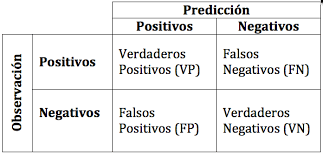
\includegraphics[width=2.5in]{images/confusion_matrix}
\end{center}
\caption{Matriz de Confusión}
\end{figure}

La estrategia solo toma la señal cuando el modelo predice un incremento en el precio, la venta por el contrario no depende del modelo, sino de los parámetros predefinidos (porcentaje de Stop Loss y Horizonte de tiempo). Esta característica implica que el valor a maximizar es la predicción de los verdaderos positivos, conocido como Precisión.

$$ Prec = \frac{VP}{VP + FN} $$

\subsection{Medidas de Riesgo}

\subsubsection{Valor en Riesgo}

El valor en riesgo ó VaR por sus siglas en inglés -Value at Risk- es una medida común del riesgo implementado en instituciones financieras. Se define como la pérdida en un portafolio, tal que existe una probabilidad $p$ que las pérdidas sean iguales o mayores que el VaR y una probabilidad $(1-p)$ que sean menores que el VaR, en un tiempo determinado. Este valor se corresponde con el cuantil de la distribución de pérdida. 

$$ Pr(Q \leq -VaR(p)) = p $$

ó

$$ p = \int_{-\infty}^{-VaR(p)}f_{q}(x)\ dx $$

siendo $f_{q}(x)$ la función de densidad de la variable aleatoria pérdida/ganancia del portafolio denotada por Q.

Aunque el VaR es utilizado comúnmente en instituciones financieras e incluso exigido en algunas regulaciones como Basilea, existen varias críticas en cuanto a su implementación. Una de las críticas es su inconclusividad en cuanto al tamaño de la pérdida, en este sentido, el VaR es un cuantil de la distribución que establece un umbral en cuanto a la posible pérdida en un período, dado un nivel de significancia. (Jon Danielsson, 2011)

\subsubsection{Pérdida Esperada}

La pérdida esperada mejor conocida conocida como 'Expected Shortfall' -ES- es una medida alternativa al VaR que responde la pregunta: ¿Cuál es la pérdida esperada cuando éstas exceden el VaR?. Formalmente la pérdida esperada se define cómo:

$$ ES = E(Q/Q \leq VaR(p)) $$ 

ó, utilizando la formulación matemática de esperanza:

$$ ES = \int_{-\infty}^{-VaR(p)} xf_{VaR}(x)\ dx $$

Es importante acotar que para el ES existen dos fuentes de error ya que primero se debe estimar el VaR y luego obtener la esperanza de la cola de la distribución. Sin embargo es una medida que complementa el VaR.  (Paff Bernhard, 2016)

En la figura 2.2 se observa la función de densidad de una distribución normal (0,1) donde se representa el VaR y ES, el VaR vendría siendo la frontera entre las dos áreas mientras que el ES la esperanza del área azul o cola superior. Es importante acotar que tanto el VaR como ES a pesar ser medidas de pérdidas potenciales, pueden ser referidas con signo negativo ó positivo.

\begin{figure}[H]
\setkeys{Gin}{height = .7\textwidth}
\centering
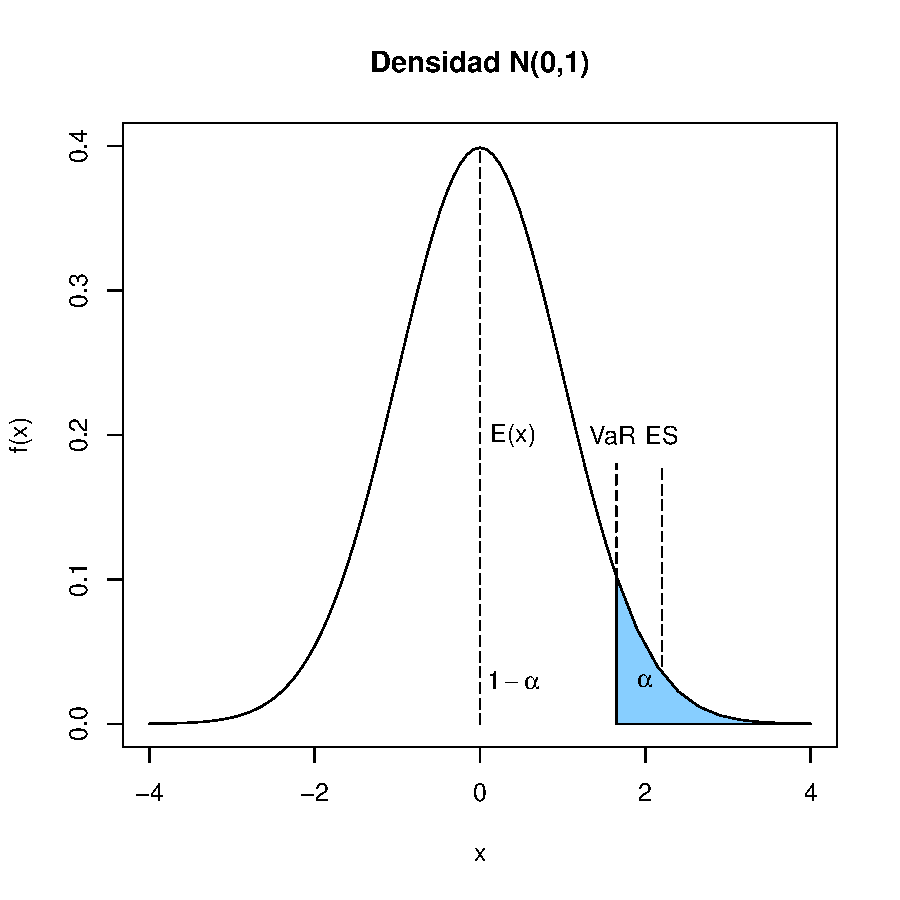
\includegraphics{main-001}
\caption{Función de densidad con VaR y ES}
\captionof*{table}{Fuente: Cálculos propios}
\end{figure}

\section{Bases Legales}

\subsection{Superintendencia Nacional de Valores}

La Ley de Entidades de Inversión Colectiva que rige las entidades de inversión en Venezuela entró en vigencia el 22 de agosto de 1996 y fue publicada en Gaceta Oficial Número 36.027. Esta se centra en entidades con capacidad de manejar importantes flujos de recurso de inversionistas hacia el mercado de capitales. El órgano encargado de autorizar, regular, controlar, vigilar y supervisar a las Entidades de Inversión y sus sociedades administradoras es la Superintendencia Nacional de Valores. (González Lisbeth, 2002)

\subsection{Basilea II y el uso del VaR para la Regulación de Entidades Financieras}

El Comité de Supervisión Bancaria de Basilea es un ente regulador que emite acuerdos para legislar la actividad bancaria. Basilea II es el segundo de estos acuerdos, fue publicado en junio de 2004 con el objeto de proteger a las entidades frente a riesgos financieros y operativos, estableciendo requerimientos de capital mínimos. Se basa en tres pilares:

\begin{itemize}
\item Requerimientos mínimos de capital: para cubrir riesgo de crédito, mercado y operacional
\item Revisión de supervisores: busca que los reguladores supervisen que las entidades mantengan reservas por encima de los requisitos mínimos y que tengan un sistema para evaluar sus riesgos.
\item Disciplina de mercado: crea incentivos para que las entidades financieras operen clara y eficientemente, siguiendo una serie de recomendaciones que buscan la publicación de movimientos financieros, perfiles de riesgo y reservas de capital
\end{itemize}

La utilización del VaR para la regulación en riesgo financiero se inicia principalmente dada las correlaciones entre los elementos de los portafolios. En 1995 se presentó un anexo sobre el modelo de riesgo de mercado, el cual autorizaba la elaboración propia del modelo de riesgo para determinar requerimientos de capital. Recomendando para la aplicación del VaR los siguientes parámetros:

\begin{itemize}
\item Horizonte de 10 días de operación o de dos semanas de calendario
\item Intervalo de confianza de 98\%
\item Un período de observación basado en un año de datos históricos actualizados, al menos una vez por trimestre
\end{itemize}
% !TeX root = ./main.Rnw
%\SweaveUTF8

\chapter{Marco Metódico}

% En el presente capítulo se describen los métodos utilizados en la investigación, con la finalidad de dar respuesta a los objetivos planteados, se indica el tipo de investigaciión, universo y muestra, la fuente donde se extraen los datos a usar y otros detalles referentes al método de estudio. De igual manera se expone la metodología para el análisis de los resultados.

\section{Tipo de Investigación}

Para definir el tipo de investigación a realizar se establece como referencia la clasificación expuesta por Balestrini (1997). La autora señala varias categorías: formulativo o exploratorio, descriptivo, diagnóstico, evaluativo, experimental ó proyecto factible. De acuerdo al problema planteado, la presente investigación es de tipo descriptivo donde se verifica que se alcancen los objetivos planteados con las conclusiones derivadas de los resultados de la simulación.

\section{Universo y Muestra}

Seijas, F. (1993) define al universo como un conjunto finito o infinito de elementos, seres o cosas. Así mismo define la muestra como un subconjunto de la población, que se obtiene para averiguar las propiedades o características de esta última, por lo que se interesa que sea representativa de la población.

El universo de estudio está representado por los índices bursátiles de los mercados financieros existentes entre el período 26/10/2008 - 18/01/2019. Un índice bursátil es un promedio de los precios de los activos que representan un mercado o sector determinado. Los mismos sirven como 'benchmark' o referencia de la economía de un país, sector financiero, etc. En el ámbito de los 'hedge funds' son una referencia para medir la rentabilidad de una estrategia de inversión y el riesgo del mercado.

En la presente investigación se utilizan los índices como reflejo del comportamiento de varios activos, de esta manera, se mide la estrategia en un sector y no en un instrumento en específico. Otras de las ventajas de utilizar los índices es que al representar un promedio de varios activos, sus variaciones son menos drásticas. La muestra está constituida por 5 índices bursátiles que representan distintos mercados del mundo: NASDAQ, NIKKEI, FTSE 100, BOVESPA y SP500.


\subsection{Tipo de Muestreo}

Seijas, F. (1993) define dos tipos de muestreo: Probabilístico y No Probabilístico.  El muestreo es probabilístico cuando se puede determinar de antemano la probabilidad de selección de cada uno de los elementos de la población siendo ésta distinta de cero; por lo tanto, calcular con antelación la probabilidad de obtener cada una de las muestras posibles.

En este caso, se realizó un muestreo no probabilístico de clase opinática, ya que la selección de los elementos de la muestra se debe a su nivel de representatividad dentro de los mercados bursátiles, por ende, la totalidad de los índices bursátiles no fueron equiprobables en su selección.

\section{Fuentes de Datos}

La estructura de los datos utilizados en el trabajo es de tipo OHLC por sus siglas en inglés Open, High, Low, Close. La misma, resume en 4 registros el comportamiento del precio del activo (Apertura, Cierre, Mínimo y Máximo) en un intervalo de tiempo. En el caso de la presente investigación, de un día. Este tipo de dato provee la información necesaria para cubrir las exigencia del modelo, tanto para la creación de la variable dependiente como para el cálculo de los indicadores técnicos.

Los datos fueron extraídos del portal www.investing.com, uno de los portales financieros con mayor prestigio en el mundo. Fue fundado en 2007 y es conocido por su calendario económico y directorio de brokers.

\section{Variables}

\subsection{Variable Dependiente}

Las decisiones de entrada en el trading pueden ser producto de muchos factores, en la presente investigación se analiza el enfoque donde se define un porcentaje objetivo de ganancia y se intenta predecir si dicho objetivo se materializa en un futuro cercano, sin que se haya concretado una venta por Stop Loss. Este enfoque reduce la toma de decisión en una variable tal que:

$$
P_{X}(x) = 
\left\{ 
\begin{array}{ll} 
p \ ; \qquad x = c
\\
\\
1-p \ ; \qquad x = -d
\end{array}
\right
$$

Dado los datos OHLC del activo es posible identificar los períodos en donde se materializa la variable dependiente. la identificación se realiza, comparando el precio de cierre con los precios máximos y mínimos de las siguientes h observaciones, donde h es el número de períodos, en este caso días en los cuales se desea evaluar la condición.

En la práctica se identifica los registros que cumplen con esta condición añadiendo una columna a la data donde incluimos 'buy' para identificar los registros donde se da la señal y 'stay' en caso de que no haya ocurrido o hubiese ocurrido primero el retroceso del precio.

\subsection{Variables Predictoras}

Los indicadores a utilizar fueron seleccionados buscando recoger la mayor información posible sobre el precio del activo, se pueden resumir en tres categorías: tendencia, momentum y volatilidad.

No es de interés en la presente investigación describir cómo funciona cada indicador para la toma de decisiones en el trading basado en fundamentos técnicos. Cada indicador puede utilizarse de distintas maneras, calcularse con distintos parámetros y asociarse a discreción del trader, lo que conlleva a un sin fin de reglas de asociación.

Lo que busca la investigación es utilizar la relación entre los indicadores como variables independientes que ayuden al modelo a predecir oportunidades de entradas. En este sentido se asume la existencia de una dinámica local del mercado que puede ser predecida con ayuda de estos indicadores. Algunos de los indicadores inicialmente escogidos para el modelo fueron excluidos debido a la alta correlación que presentan. A continuación se exponen los indicadores utilizados:

\begin{itemize}
\item Retornos con respecto al precio de Cierre.
\item RSI (Relative Strength Index) de 14 períodos, el cual es un indicador de volatilidad.
\item MACD (Moving Average Converge/Divergence) el cual es una diferencia de dos EMAs (Exponential Moving Average) de 12 y 26 períodos. Este es un indicador de tendencia que se complementa con un EMA de 9 períodos. 
\item ADX (Average Directional Index), este es un indicador que utiliza dos indicadores de dirección +Di y -Di, se calculó en base a 14 períodos y mide tendencia.
\item Bandas de Bollinger, el cual es un indicador de tendencia y volatilidad, utiliza dos bandas calculadas a partir de una media móvil con desviaciones estándar. Se utilizó en base a 14 períodos y una desviación de 2.5.
\item ATR (Average True Range), es un indicador de volatilidad calculado a partir de los máximos y mínimos de un período, en este caso 14.
\end{itemize}

Estos indicadores están fuertemente correlacionados por lo que se decidió, disminuir el número de variables dejando solo las más representativas de cada indicador.

Ahora bien, la idea base de la investigación era utilizar los valores de cada indicador como variables predictora. Dado que el cálculo de todos los indicadores provienen de la misma variable -precio del activo, en la mayoría de los casos precio de cierre-, existe una alta colinealidad entre ellos, la idea de utilizar el ACP es precisamente para enfrentar este problema como se detalla más adelante. Sin embargo, es de notar que los valores de los indicadores por sí solos no proveen un poder predictivo, lo que realmente usa el trader son las asociaciones entre indicadores para encontrar patrones. 

Se decidió entonces, utilizar como predictores no los indicadores por si solos, sino, las relaciones entre cada uno de ellos. Esto se abordó agregando al modelo las interacciones entre todos los indicadores, y removiendo los valores de los indicadores por sí solos. De esta manera el hecho de utilizar ACP, no solo es utilizado para remover la colinealidad entre predictores, sino, como método de reducción de variables, ya que el modelo pasó de tener 10 predictores -incluyendo el precio de cierre- a 45.

\section{Estrategia de Análisis}

\subsection{WalkForward Backtesting}

Al principio de la investigación se implementó el método de entrenamiento, validación y prueba comúnmente utilizado, en donde la mayor parte de la data es destinada a entrenamiento del modelo, otra sección es destinada a validación, para elegir los parámetros óptimos, y finalmente se aplica el modelo en la data de prueba. Sin embargo este tipo de metodología en opinión del investigador no es el más óptimo para desarrollar el presente modelo, ya que el dinamismo de los mercados bursátiles no permite al algoritmo permanecer sin cambios en el tiempo.

Para contrarrestar esta situación se optó por el método de backtesting Walkforward, el cual consiste en entrenar el modelo en un período base de data, en este caso los primeros 4 años de estudio, posteriormente se aplica la estrategia en el año siguiente y se obtiene los primeros resultados. Luego este año de aplicación es incluído en la data de entrenamiento -es decir, la data de entrenamiento pasa a ser de 5 años- y se evalúa el modelo en el siguiente año. De esta manera, contemplamos el dinamismo del mercado permitiéndole al modelo -y por ende a la estrategia- utilizar el período más reciente con respecto al cual será implementado. En la presente figura 3.1 se ilustra la metodología implementada.

\begin{figure}[ht]
\begin{center}
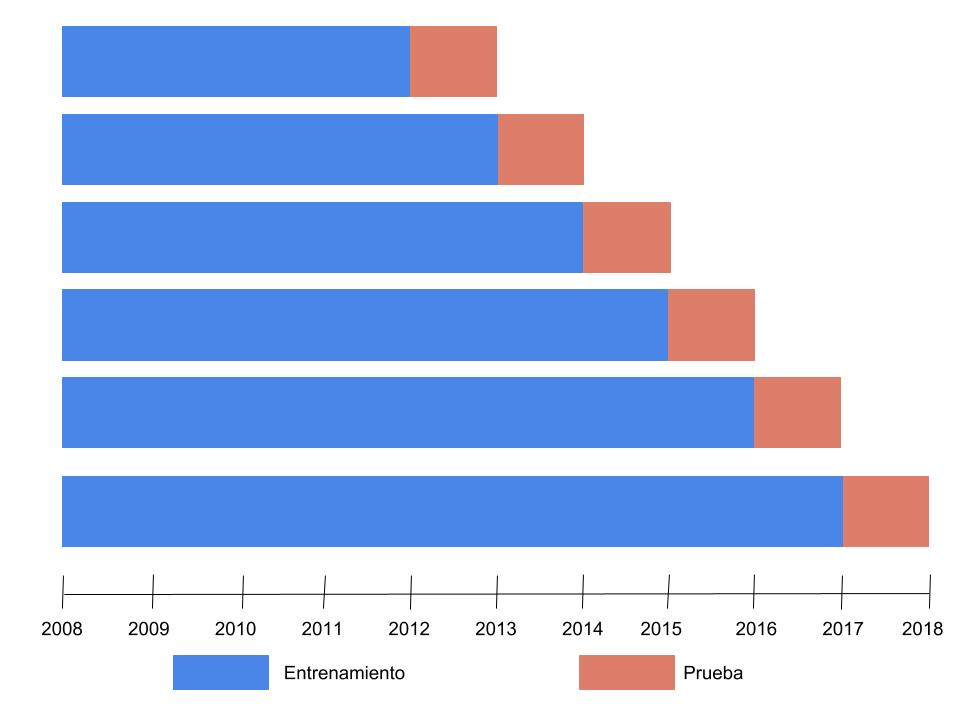
\includegraphics[width=3in, height=3in]{images/walkforward_plot}
\end{center}
\caption{Metodología WalkForward}
\captionof*{table}{Fuente: Cálculos propios}
\end{figure}

Otra de las características de la metodología que se modificó fue la elección de los valores de los hiperparámetros -target, stop y horizonte-. Previamente se utilizaba la data de validación para buscar la combinación de parámetros óptima. Ahora bien en la metodología de Walkforward se utilizan los mismos parámetros durante todo el período de estudio. A opinión del investigador al buscar los mejores parámetros se estaría incurriendo en un posible sesgo de sobreoptimización. El hecho de que en un año determinado unas configuraciones den los mejores resultados no asegura que se replique en el siguiente año.

Por otro lado, si se utiliza un stop ó target muy altos, baja el número de observaciones que cumplan con la condición de la variable dependiente, por lo tanto se estaría en presencia de un problema de data desequilibrada que debe tener un tratamiento distinto. En base a esto, se establece el target en 2\% y el stop en 2,5\%. Por otro lado la elección del horizonte de tiempo influye también en el número de observaciones identificadas como 'buy', es de notar que mientras más grande el horizonte mayor número de observaciones 'buy' se tendrá. Sin embargo existe un punto en donde deja de crecer este número, en la práctica se establece en 20. En la figura 3.2 se ilustra el número de observaciones identificadas como 'buy' para distintas combinaciones de hiperparámetros.


\begin{figure}[H]
\setkeys{Gin}{width = 0.8\textwidth}
\centering
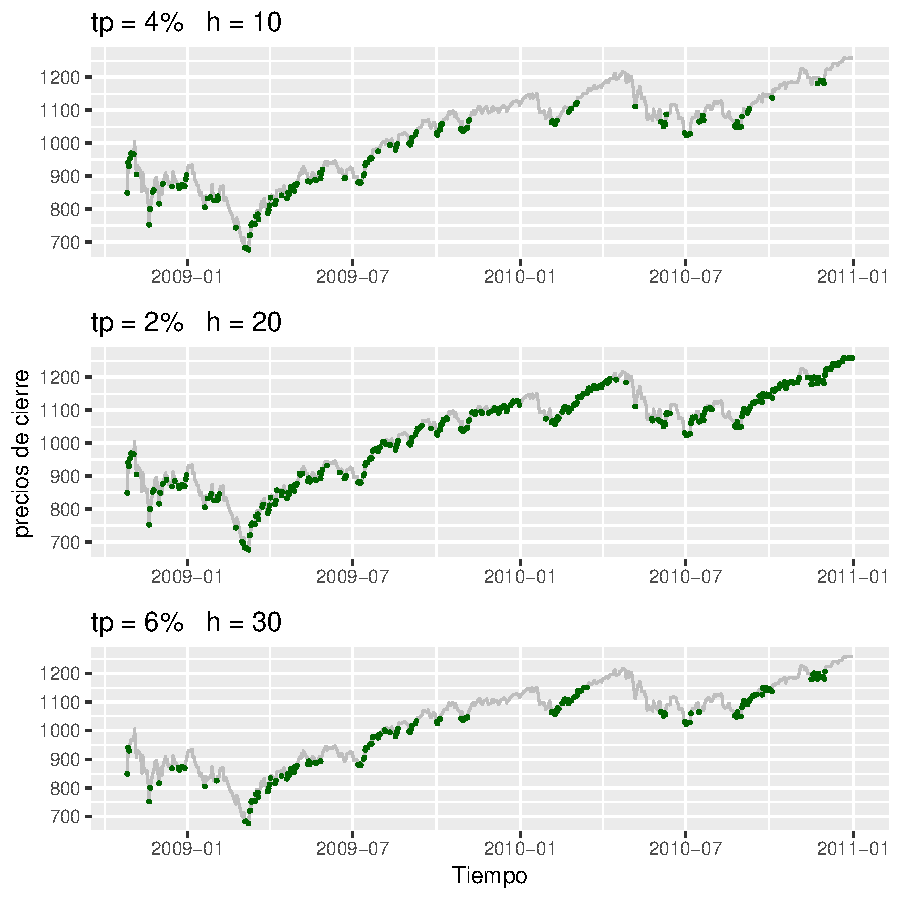
\includegraphics{main-003}
\caption{Observaciones que presentan ocurrencias con sl = 2.5\%, en el primer conjunto de datos de entrenamiento (26/10/2008 - 31/12/2010) para el índice S\&P500, para diferentes valores de tp y h}
\captionof*{table}{tp = Take Profit, sl = Stop Loss, h = Horizonte. }
\captionof*{table}{Fuente: Cálculos propios}
\end{figure}

\subsection{Regresión Logística}

Los modelos lineales generalizados asumen que existe una aproximada relación lineal entre la variable respuesta $Y$ y la variables predictoras $X$. Matemáticamente se puede describir la relación como:

$$ Y \approx \beta_{0} + \beta_{1}X_{1} + ... + \beta_{j}X_{j} $$

En donde $X_{j}$ representa las variables predictoras y los coeficientes $\beta_{j}$ cuantifican la asociación entre la variable predictora $X_{j}$ y la variable respuesta $Y$. Por lo que se interpreta a $\beta_{j}$ como el efecto promedio que tiene en $Y$ un incremento de una unidad en $X_{j}$, bajo el supuesto de que todas las demás variables se mantienen constantes.

% En problemas de clasificación, la variable predictora asume valores categóricos, por lo que al utilizar este enfoque se pueden obtener probabilidades fuera del intervalo [0, 1], haciendo imposible su interpretación. Esto concluye en que se deba utilizar una función, tal que permita la generación de valores entre [0, 1], en el caso de la regresión logística esta función es:

En problemas de clasificación, la variable predictora asume valores categóricos, por lo que se necesita una función que arroje probabilidades propias de esta labor, en el caso de la regresión logística esta función es:

$$
p(X) = \frac{e^{\beta_{0} + \beta_{1}X_{1} + \beta_{2}X_{2} + ... + + \beta_{j}X_{j} }}{1 + e^{\beta_{0} + \beta_{1}X_{1} + \beta_{2}X_{2} + ... + + \beta_{j}X_{j} }}
$$

Despejando se obtiene

$$ \frac{p(X)}{1 - p(X)} = e^{\beta_{0} + \beta_{1}X_{1} + \beta_{2}X_{2} + ... + + \beta_{j}X_{j} } $$

El lado izquierdo de la ecuación puede tomar valores entre 0 e $\infty$, lo cual indicaría muy bajas o muy altas probabilidades, aplicando logaritmo en ambos miembros de la ecuación se obtiene la función logit.

$$ \log{\frac{p(X)}{1 - p(X)}} = \beta_{0} + \beta_{1}X_{1} + \beta_{2}X_{2} + ... + + \beta_{j}X_{j}  $$

Se observa que la función logit es lineal en $X$, por lo que incrementar una unidad de $X$ afecta el lado izquierdo de la ecuación en $\beta$. Sin embargo dado que la relación entre $p(X)$ y $X$ no es una línea recta, $\beta$ no corresponde a un cambio en $p(X)$ asociado a una unidad de incremento en $X$. Se debe hacer la respectiva transformación para interpretar el coeficiente $\beta$ en relación a $Y$.

% \subsubsection{Máxima Verosimilitud}
% 
% Los coeficientes $\beta$ son desconocidos, por lo que deben estimarse en la data de entrenamiento. Para esto se utiliza el método de $Máxima Verosimilitud$, el cual consiste en estimar los coeficientes para los cuales la probabilidad de predicción para cada individuo, utilizando (fórmula arriba), corresponda lo más cercano posible al valor observado del individuo. Se define la función de verosimilitud como
% 
% $$ l(\beta) = \prod_{i=1}^{j}{P(x_{i} / \beta)} $$
%   
% Por conveniencia se  trabaja con el logaritmo, dado que esto transforma una operación de productos de probabilidades en una sumatoria, por lo que se obtiene
% 
% $$ l(\beta) = \sum_{i=1}^{N} \log{P(y_{i}/ x_{i}; \beta)} $$
% 
% Al codificar las clases en 0 y 1, la función de verosimilitud para la regresión logarítmica puede ser escrita como
% 
% $$ l(\beta) = \sum_{i=1}^{N}(y_{i}\beta^{T}x_{i} - \log{1 + e^{\beta^{T}x_{i}}}) $$
% 
% Para maximizar la función, se iguala la derivada a 0
% 
% $$ \frac{\partial l(\beta)}{\partial \beta} = \sum_{i=1}^{N}x_{i}(y_{i} - P(x_{i}; \beta)) = 0 $$
% 
% Para resolver la ecuación (n arriba) se utiliza un algoritmo de optimización llamado $Newton-Raphson$

\subsection{Reducción de la dimensión con ACP}

La técnica que utiliza el análisis de componentes principales (PCA) para reducir el número de variables predictoras es conocido como Principal Component Regression (PCR). PCR es utilizado para extraer la información más importante de una matríz de datos multivariante y expresar ésta información en nuevas variables llamadas componentes principales, éstas son una combinación lineal de las variables originales. Aunque el número de componentes principales puede ser igual al número de variables, la idea es utilizar un grupo reducido de componentes que maximicen la variación.

Por su parte el modelo propuesto utiliza las interacciones entre las variables predictoras, esto aumenta el número de variables de 10 a 45, las cuales además en muchos casos están correlacionadas. Al utilizar PCR se reduce el número de variables a dos componentes que contienen alrededor del 50\% de la variación, es importante recordar que esta reducción se realiza en cada período de entrenamiento.

\subsection{Modelado de los Retornos}

Tal como se establece en la sección 3.1.3 la variable aleatoria retorno del trade puede obtener 2 posibles valores, si el trade es exitoso toma el valor c con probabilidad p, en caso contrario toma el valor -d con probabilidad 1-p. 

$$
P_{X}(x) = 
\left\{ 
\begin{array}{ll} 
p \ ; \qquad x = c
\\
\\
1-p \ ; \qquad x = -d
\end{array}
\right
$$

Para cada activo se puede asumir p como la probabilidad positiva -precisión- obtenida en el modelo. Por su parte c y -d son fijados en 200 y -250 respectivamente, esto viene dado por haber establecido los porcentajes de salida en 0.02 de ganancia y 0.025 de pérdida y asumir un capital a riesgo en cada trade de 10.000 USD.

Asumiendo que la ocurrencia de los trades es una variable aleatoria i.i.d, es posible aplicar el teorema central del límite. Con un número de muestra suficientemente grande, la suma de estas variables se aproxima una distribución normal 0,1.

$$ \frac{\sum x_{i} - nE(x)}{\sqrt{n}\sigma_{x}} \sim N(0,1) $$

siendo

$$ E(x) = pc - (1-p)d \qquad y \qquad \sigma^{2}_{x} = (pc^{2} - (1-p)d^{2}) - (pc - (1-p)d)^{2} $$

Es posible modelar los retornos producidos por la estrategia y calcular el valor a riesgo -VaR- y pérdida esperada -ES- dado un número de operaciones. Tanto el VaR como el ES son medidas comúnmente utilizadas para representar el riesgo de pérdida en un período de tiempo determinado, en este caso, se establecerá en vez de tiempo, un número de trades cerrados por la estrategia.

Dado que el retorno de la estrategia se distribuye N(0, 1), se definen el VaR y ES cómo

$$ VaR_{\alpha} = \sigma \Phi^{-1}(\alpha) - \mu $$

$$ ES_{\alpha} = \sigma \frac{\phi(\Phi^{-1}(\alpha))}{1-\alpha} - \mu $$

En la presente investigación se establecen $n = 300$ y $\sigma = 0.95$. Es decir que el VaR puede interpretarse como: ''Existe una probabilidad del 5\% que la estrategia genere una pérdida igual ó menor que $VaR_{\alpha}$, luego de 300 trades realizados''.

Mientras que el ES se interpreta como: ''En caso de que la estrategia genere una pérdida mayor que $VaR_{\alpha}$ luego de 300 trades, se espera que ésta pérdida sea de $ES_{\alpha}$''
% !TeX root = ./main.Rnw
%\SweaveUTF8

\chapter{Análisis de Resultados}

\section{Análisis Exploratorio de los datos}

En el presente capítulo se realiza la descripción de los resultados obtenidos luego de la aplicación del método propuesto para la simulación de la estrategia. De igual modo, se presentan los coeficientes arrojados por el MLG así como un analisis de los componentes principales para el índice S\&P500 


\subsection{Análisis de los Índices}

En la figura 4.1 se observa el precio de cierre de cada índice durante el período de estudio. Se puede apreciar que en general los cinco mercados tienen tendencia a la alta. En general para el S\&P y NASDAQ se aprecia una menor variabilidad que en los demás índices.

La crisis de la burbuja inmobiliaria en Estados Unidos afecto significativamente a todos los mercados del mundo, la mayoría de los índices alcanzaron mínimos en octubre de 2008 y desde ese momento fueron incrementandose nuevamente, por eso vemos un patrón alcista en los 5 índices, debido a que un año antes muchos habían perdido hasta 60\% de su valor.

Las curvas del S\&P y NASDAQ son muy parecidas ya que ambas representan cotizaciones de las mayores empresas americanas. Se aprecia un crecimiento sostenido desde el año 2009, con algunos períodos más estables, a principios del 2016 -por la polémica victoria de Donald Trump como presidente- y en 2018 provocado por el miedo a un incremento en las tasas de interés por parte de la Reserva Federal y las tensas negociaciones con China.


\begin{figure}[H]
\setkeys{Gin}{width = 0.8 \textwidth}
\centering
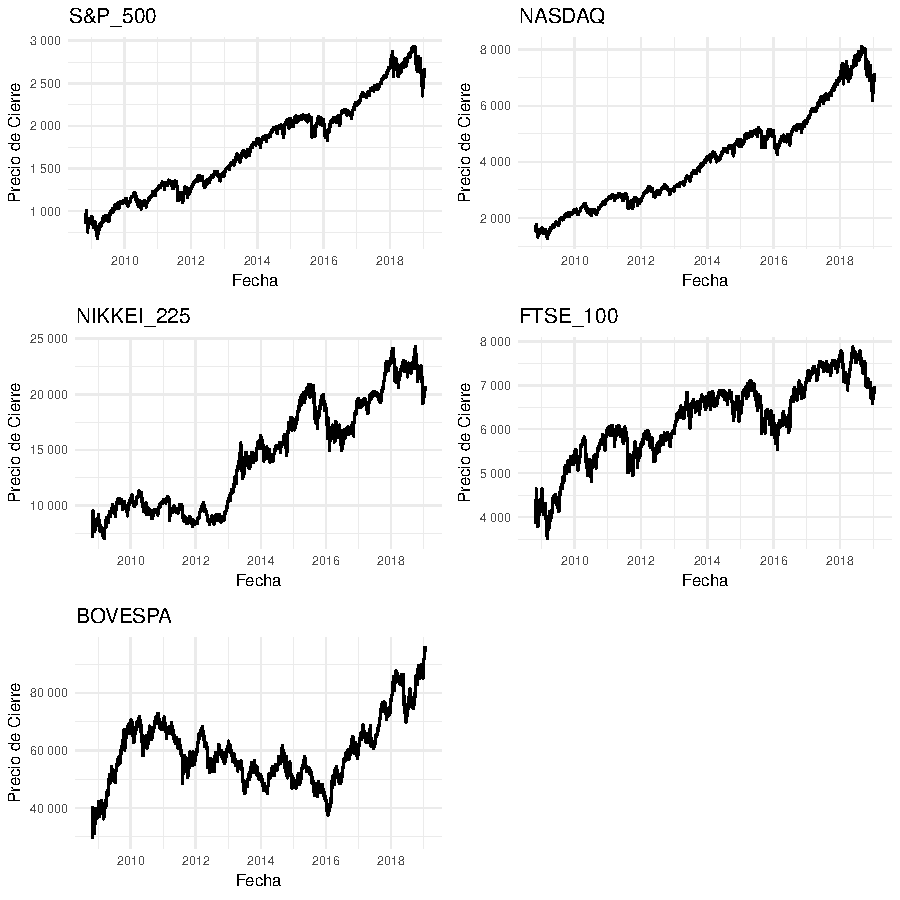
\includegraphics{main-005}
\caption{Precios de Cierre de los índices en el período de estudio (26/10/2008 - 18/01/2019)}
\captionof*{table}{Fuente: Cálculos propios}
\end{figure}

Por su parte, al ver la gráfica del NIKKEI se observa un rápido crecimiento entre 2009 y 2010, sin embargo con la ocurrencia del terremoto registrado en el norte del país a principios del 2011 el índice se vio afectado y llegó a su nivel más bajo de 8160 puntos el 25 de noviembre desde el 10 de marzo de 2009. La recuperación ocurrió en 2013 debido a los cambios implementados por el país en materia de política fiscal y monetaria. El Gobierno impulsó el gasto público y el Banco Central de Japón inyectó dinero en la economía a gran escala.

El FTSE 100 es un índice bursátil calculado con las cotizaciones de las 100 empresas más grandes de Reino Unido, en su gráfica se observa una tendencia alcista aunque con mayor ruido o variabilidad que los otros índices. Se puede apreciar una caída en las cotizaciones el año 2015 debido a resultados negativos mostrados por la actividad manufacturera en Asia, especialmente en China. Esto afecta los mercados europeos dado que este es el principal consumidor del mercado asiático.

Por último en las cotizaciones del índice BOVESPA se aprecia que, a diferencia de los anteriores, mantiene una tendencia a la baja hasta 2016 debido a la recesión económica sufrida por Brasil mostrando una contracción del PIB en un 3.8\% para 2015. Aunado a factores ambientales como el virus del Zika y el escándalo de corrupción de Petrobras. A partir de 2016 con la inflación gradualmente bajo control y tasas de interés en decrecimiento, la confianza de los inversores llevó a un rápido crecimiento del índice en los últimos tres años.

\subsection{Análisis de las Variables Predictoras}

En la figura 4.2 se refleja la correlación de las variables originales para el primer período de entrenamiento del índice S\&P500. Como se puede observar existe alta correlación entre las distintas variables del precio (Apertura, Cierre, Máximo y Mínimo) por lo que se decidió trabajar solo con los precios de cierre dado que ésta es la misma utilizada para determinar la variable dependiente. Así mismo se observa alta correlación entre los rezagos de los rendimientos, para esto se decidió trabajar solo con los rezagos de 1, 3 y 5 períodos. Se descarta la variable dip -elemento utilizado en el indicador ADX- por su fuerte correlación con el RSI. Se determina lo mismo para la banda inferior del indicador de Bollinger. En la figura 4.3 se muestra las correlaciones de las variables definitivas

\begin{figure}[H]
\setkeys{Gin}{width = 0.6\textwidth}
\centering
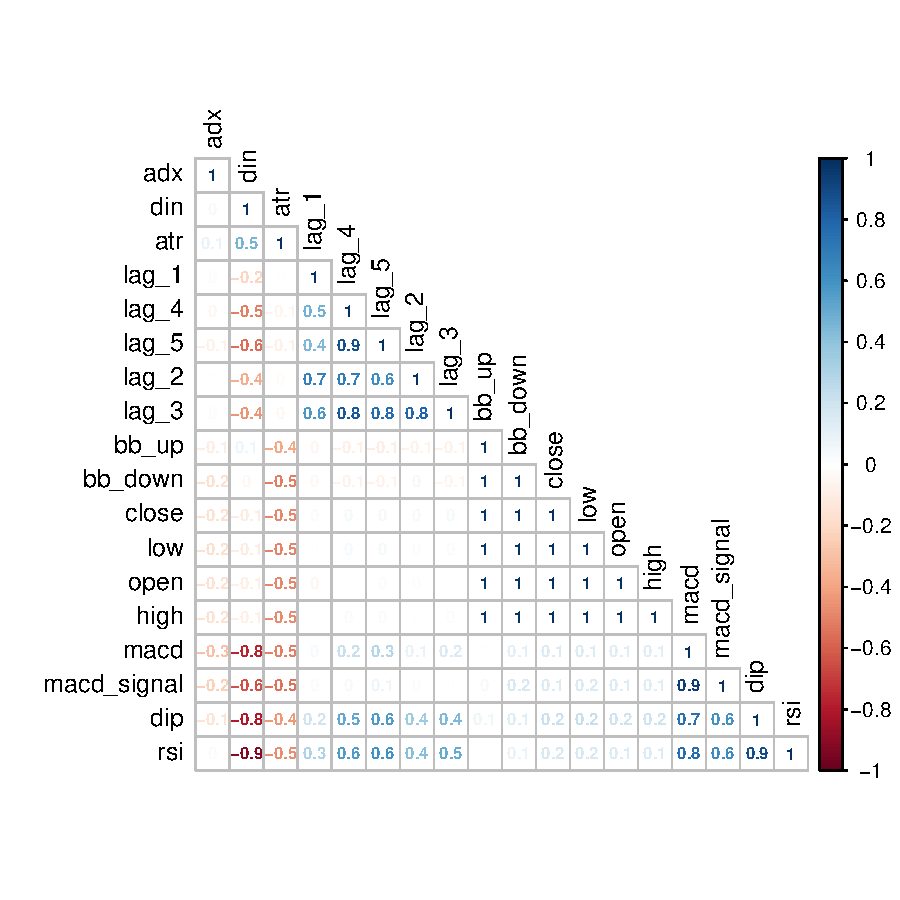
\includegraphics{main-006}
\caption{Correlación entre indicadores originales calculados con los precios del S\&P500 en el primer período de entrenamiento(01/01/2009 - 31/12/2012)}
\captionof*{table}{Fuente: Cálculos propios}
\end{figure}

\begin{figure}[H]
\setkeys{Gin}{width = 0.6\textwidth}
\centering
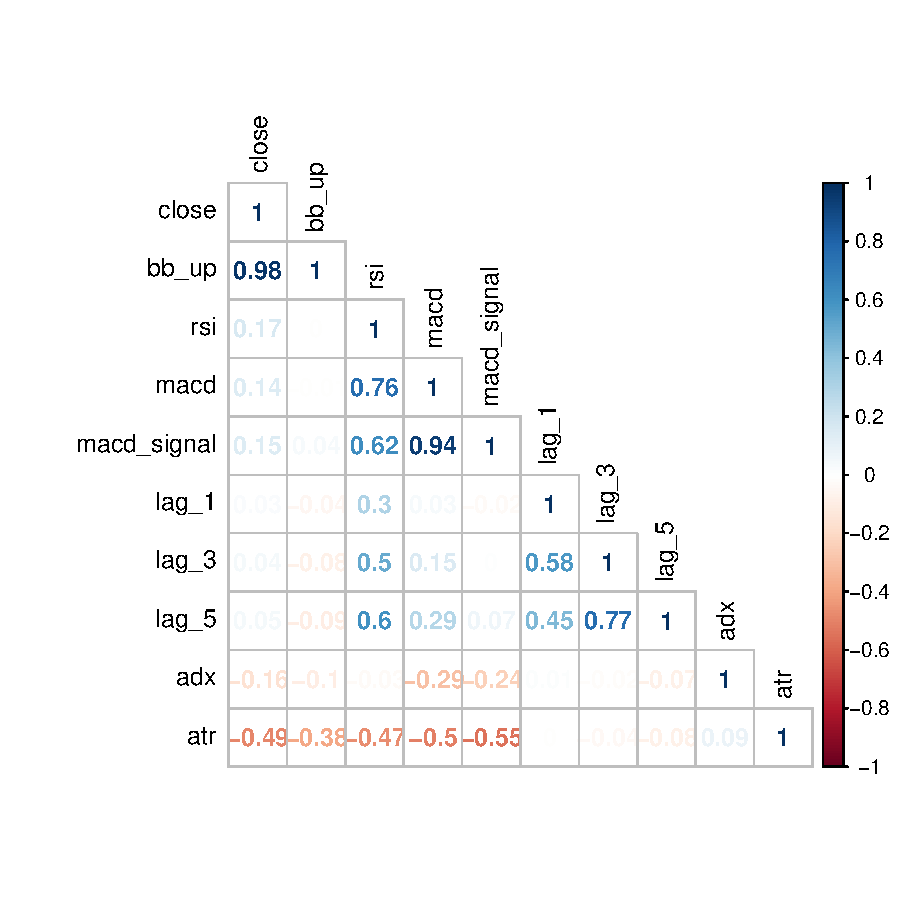
\includegraphics{main-007}
\caption{Correlación entre indicadores definitivos calculados con los precios del S\&P500 en el primer período de entrenamiento(01/01/2009 - 31/12/2012)}
\captionof*{table}{Fuente: Cálculos propios}
\end{figure}

A continuación se presentan una serie de gráficos para reflejar lo anteriormente expuesto en cuanto a la relación entre los indicadores.


\begin{figure}[H]
\centering
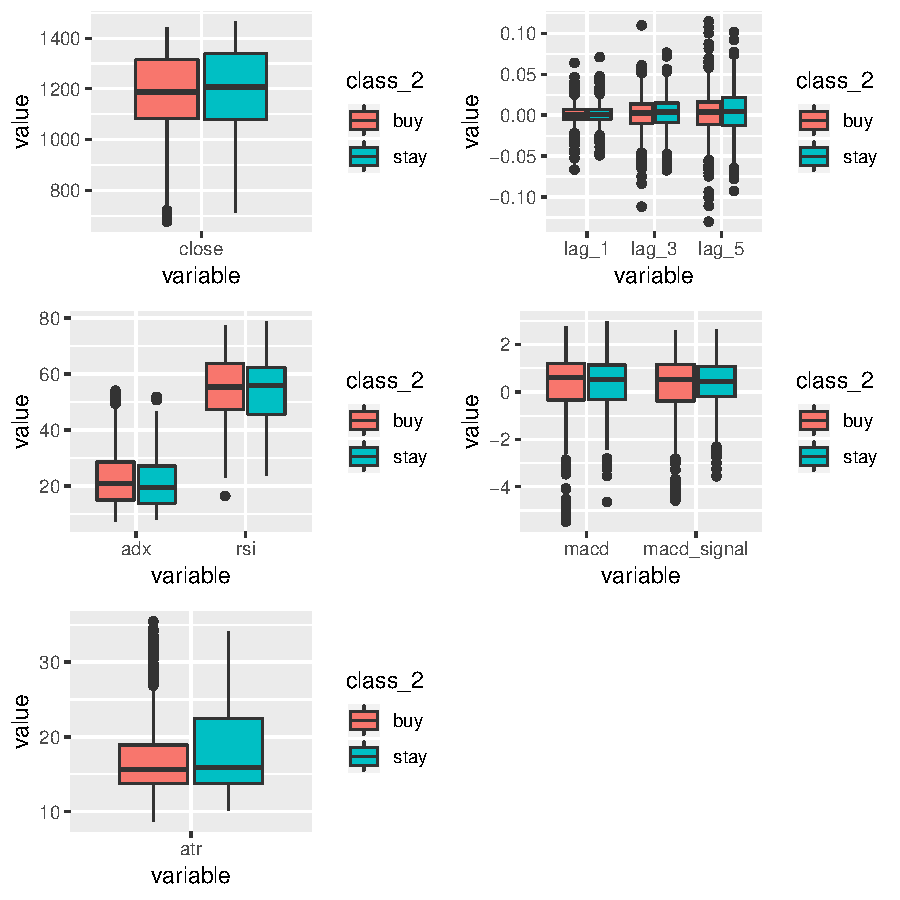
\includegraphics{main-009}
\caption{Gráfico de cajas de indicadores definitivos calculados con los precios del S\&P500 en el primer período de entrenamiento(01/01/2009 - 31/12/2012)}
\captionof*{table}{Fuente: Cálculos propios}
\end{figure}

En la figura 4.4 se observan gráficos de cajas para cada una de las variables predictoras, diferenciando entre los registros identificados como 'buy' y 'stay'. En el caso de la variable close, se aprecia que tanto el tercer cuartil como la mediana están ligeramente mas abajo para los registros marcados como 'buy', señalando que efectivamente las entradas ocurren a precios bajos. En el caso de los rezagos -lags- se observa que mientras mayor sea el número de períodos para su cálculo, mayor diferencia existirá entre el primer y tercer cuartil y entre los valores atípicos, lo que se traduce en mayor dispersión y variabilidad entre las clases.

Para la variable ADX el primer, segundo y tercer cuartil de los registros 'buy' está ligeramente más arriba que los 'stay' lo que indicaría que se debería comprar en tendencia alcista. Igualmente ocurre con la variable RSI lo que indicaría que se compra cuando se está cerca de un cambio de tendencia ó por el contrario la consolidación de la misma. Para la variable ATR se observa como el tercer cuartil de los registros identificados como 'buy' esta más abajo y hay menos dispersión, por lo cual se inferiría que se debe comprar en períodos de baja volatilidad.

\begin{figure}[H]
\centering
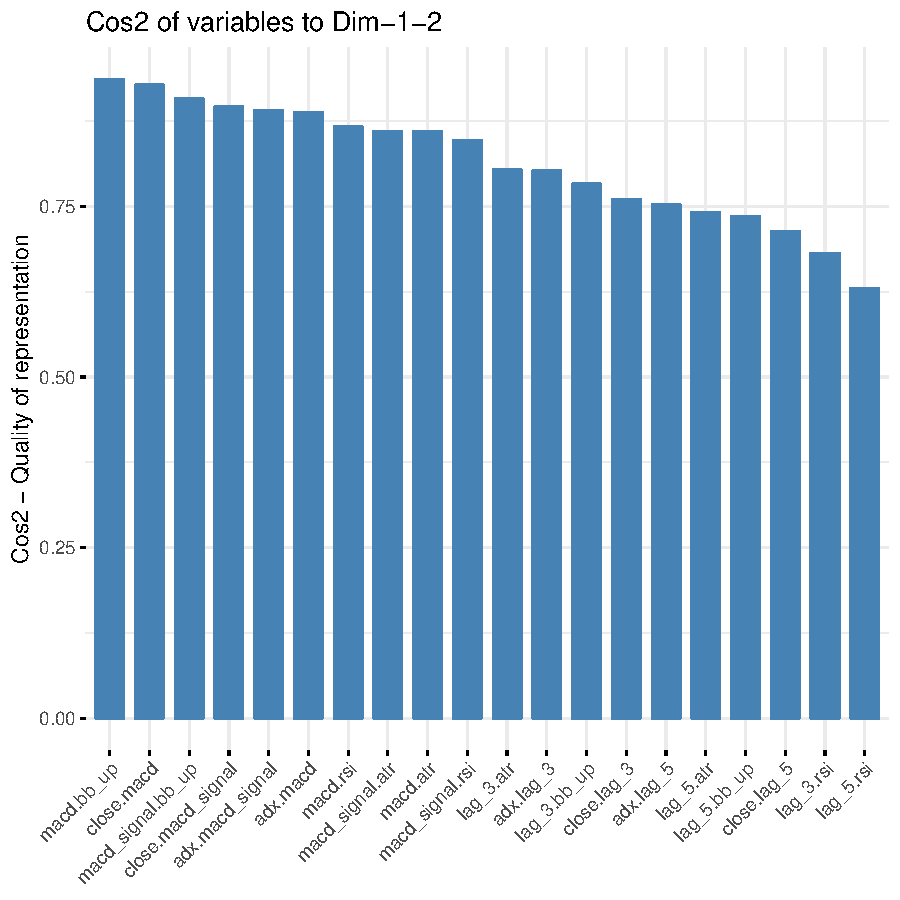
\includegraphics{main-010}
\caption{Histogramas de frecuencia de indicadores definitivos calculados con los precios del S\&P500 en el primer período de entrenamiento(01/01/2009 - 31/12/2012)}
\captionof*{table}{Fuente: Cálculos propios}
\end{figure}

En la figura 4.5 se exponen histogramas de frecuencias para cada indicador. Se observa como la distribución de los rezagos es similar entre ellos, mostrando datos simétricos con mayor frecuencia en los valores cercanos a 0. En cuanto a la variable ATR se observa que los datos son asimétricos hacia la derecha con algunos casos atípicos cercanos a 30, mostrando que el índice en general es de baja volatilidad. Para el caso de la banda de bollinger, sigue una distribución muy parecida a la del valor de cierre de precio, una distribución plateau con una ligera asimetría hacia la izquierda lo que referencia en general una tendencia alcista. Por otro lado el ADX muestra una distribución asimétrica hacia la derecha con valores entre 10 y 20 lo cual indicaría que esta tendencia alcista del índice es constante pero lenta. 

La distibucion de la variable RSI es asimétrica hacia la izquierda con la mayor frecuencia entre los valores cercanos a 60, lo cual reforzaría lo indicado por los otros indicadores en cuanto a la tendencia del índice.

\begin{figure}[H]
\centering
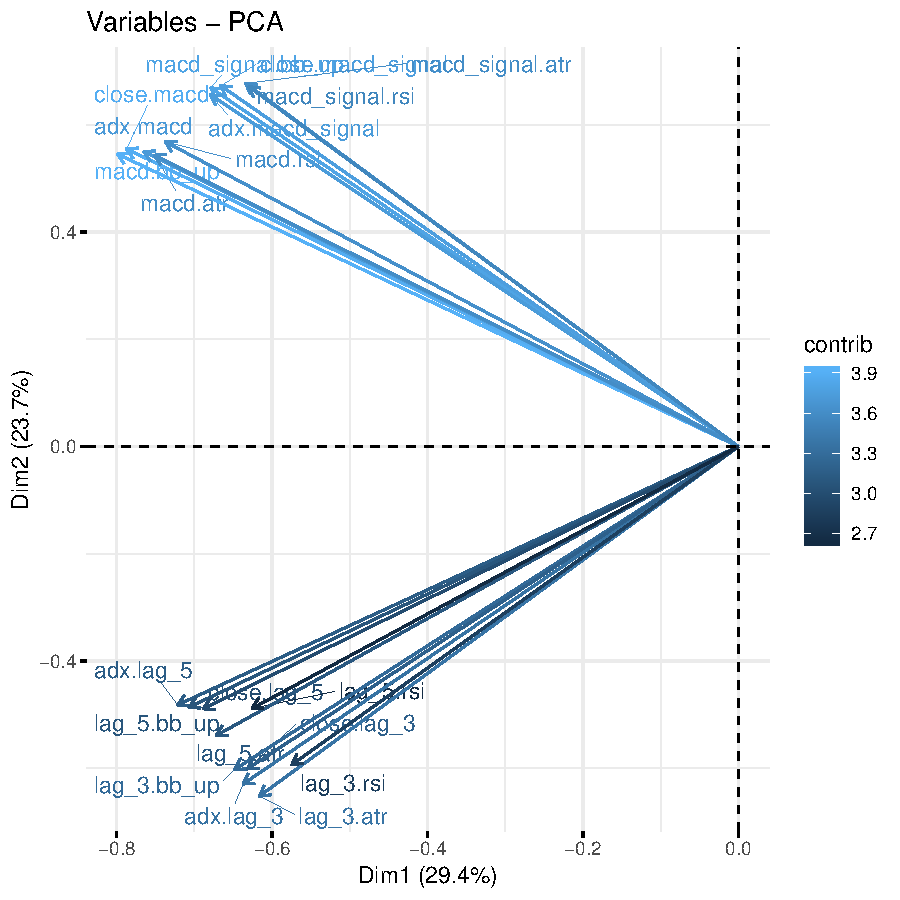
\includegraphics{main-011}
\caption{Gráfico de densidad de indicadores definitivos calculados con los precios del S\&P500 en el primer período de entrenamiento(01/01/2009 - 31/12/2012)}
\captionof*{table}{Fuente: Cálculos propios}
\end{figure}

En la figura 4.6 se observan gráficos de densidad para cada variable diferenciando entre clases, buscando algún comportamiento diferenciador. Sin embargo se muestra como para todos los indicadores la densidad es muy similar entre clases.

\subsection{Resultados del ACP}

A continuación se analizan los resultados de los componentes arrojados por el modelo en el primer período de entrenamiento (2009-2012) utilizando el índice S\&P500, en esta sección se referirá a ésta como 'matriz de datos'. Ahora bien, si se quisiera analizar cada una de las componentes arrojadas en cada muestra de entrenamiento se necesitaría repetir este análisis 30 veces lo cual no es práctico para los fines de la investigación. En este sentido se elaboró una aplicación con el paquete Shiny del programa R, para visualizar de manera interactiva las gráficas que ayudan a entender los componentes. La aplicación puede ser visitada con el siguiente enlace \url{https://rodserr.shinyapps.io/trading-ML/}. En dicha plataforma es posible cambiar el índice al cual se quiere hacer referencia al igual que la ventana de entrenamiento, se pueden observar tanto las gráficas de correlación de los componentes como la gráficas de los autovalores y variabilidad explicada.


Los autovalores miden la cantidad de variación retenida por cada componente. Los autovalores son mayores para los primeros componentes, dado que el primer componente busca maximizar la cantidad de variación de la matriz de datos, por lo que cada vez es menor la cantidad de variación retenida por cada componente.

\begin{figure}[H]
\setkeys{Gin}{width = 0.8\textwidth}
\centering
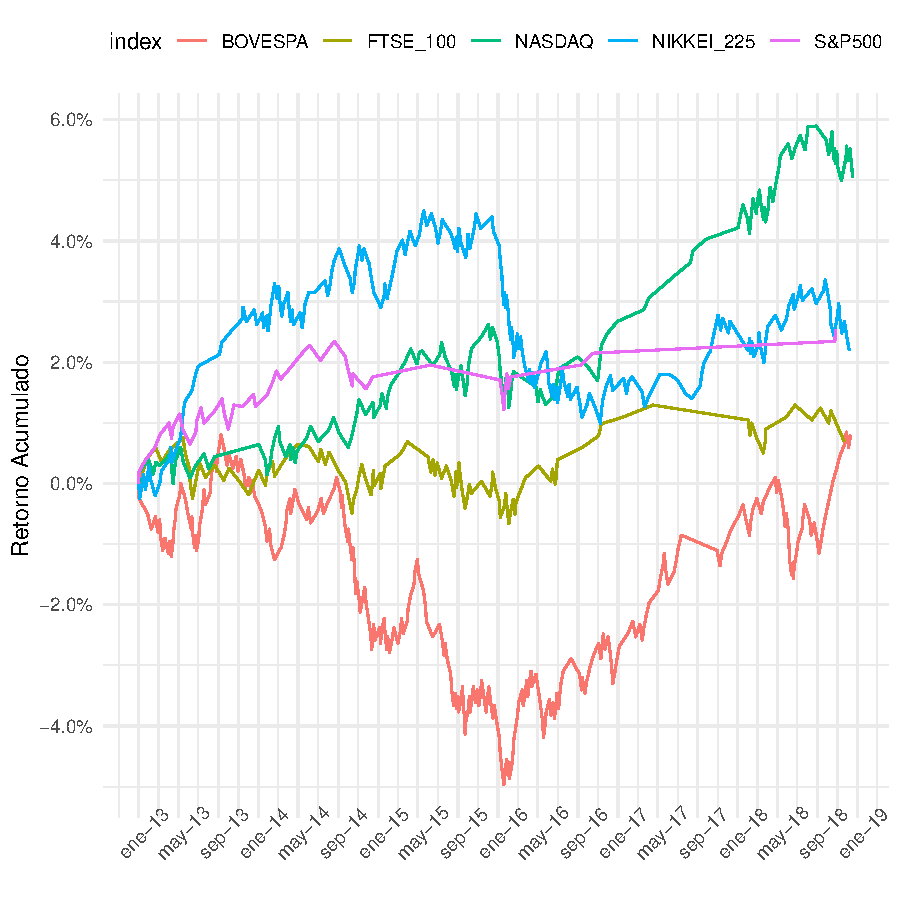
\includegraphics{main-013}
\caption{autovalores y Porcentaje de contribución para los 10 componentes más importantes obtenidos por la matríz de datos}
\captionof*{table}{Fuente: Cálculos propios}
\end{figure}

La proporción de variación explicada por cada autovalor viene dada de dividir cada autovalor por su sumatoria, en este caso 45 -el número de variables originales-. Un autovalor mayor que 1 indica que el componente tiene mayor variación que la contenida en una de las variables originales. En la figura 4.7 se puede observar que el 85\% de la variación está contenida en los primeros 7 componentes. Igualmente se aprecia que el autovalor de los 10 PCs es mayor que 1. 

El número de componentes a utilizar se establece en función a estos dos gráficos. Este comportamiento anteriormente descrito se replica en los demás períodos de entrenamiento y demás pares. Se decide utilizar los dos primeros componentes como variables explicatorias en el MLG ya que la diferencia entre el 2do y 3er componentes es significativa, por lo que se espera que la variabilidad explicada en los dos primeros componentes -aproximadamente 50\%- sea suficiente. Esto también se basa en el hecho de que los indicadores son transformaciones del precio del activo por lo que existe correlación entre ellos. Se asume entonces que no es necesaria toda la información provista por los indicadores.

La contribución de las variables representan la variabilidad contenida en un componente. Las variables correlacionadas con el componente principal 1 (PC1) y componente principal 2 (PC2) son las más importantes en explicar la variabilidad en la matriz de datos. Aquellas que no se correlacionan con ninguna componente son desechadas por su baja contribución. En la figura 4.8 se observa la contribución de las primeras 30 variables en PC1, PC2 y la contribución obtenida en ambas.

\begin{figure}[H]
\setkeys{Gin}{width = 0.8\textwidth}
\centering
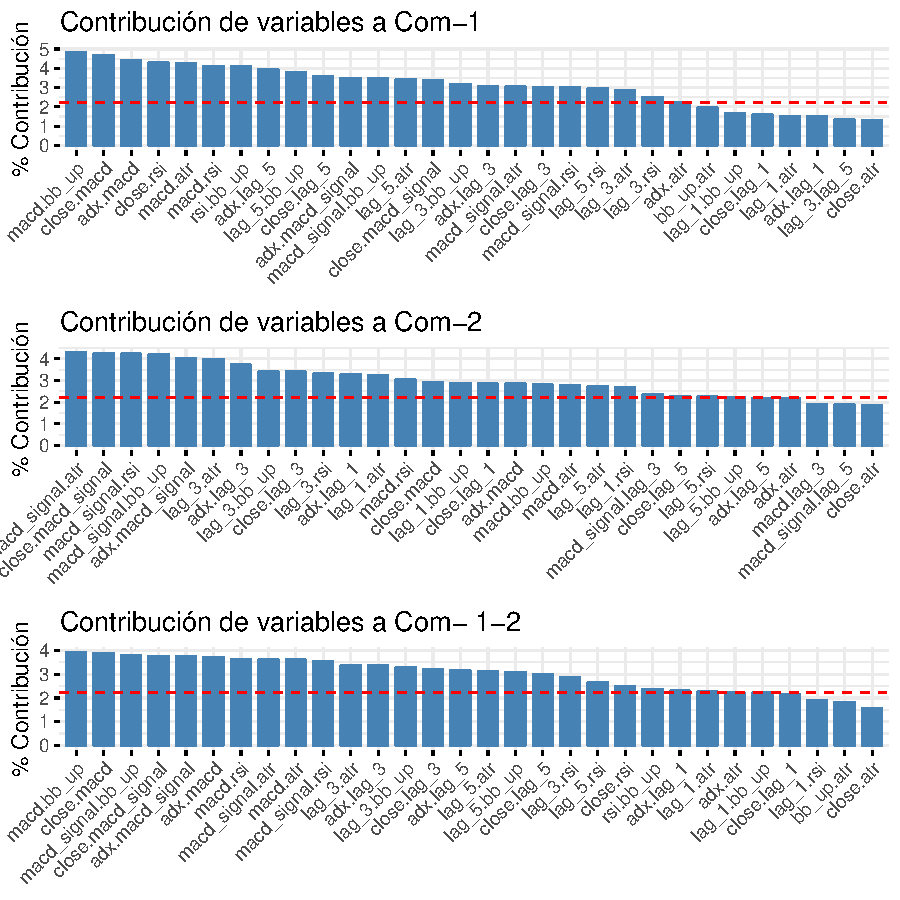
\includegraphics{main-014}
\caption{Contribución de cada variable para PC1, PC2 y el total de la contribución en ambos componentes}
\captionof*{table}{Fuente: Cálculos propios}
\end{figure}

La línea roja indica el promedio esperado de contribución si las variables fueran uniformes, es decir $ \frac{1}{N° de Variables}x100 = \frac{1}{45}x100 = 2,2\%$. Una variable sobre este umbral se considera importante en la contribución al componente. Se aprecia cómo las interacciones que predominan en ambos componentes están relacionadas con el indicador MACD.

La calidad de representación en el gráfico viene dada por el valor de $Cos^2$, el cual se refiere a la importancia que tiene la variable para interpretar el componente. Para una variable la suma de $Cos^2$ en todas las componentes equivale a 1. En la figura 4.9 se muestra los valores de $Cos^2$ para las primeras 2 componentes, se puede observar que las variables que mejor representan a los componentes son las interacciones de los indicadores MACD con otros indicadores, así como las interacciones de los rezagos.

\begin{figure}[H]
\setkeys{Gin}{width = 0.8\textwidth}
\centering
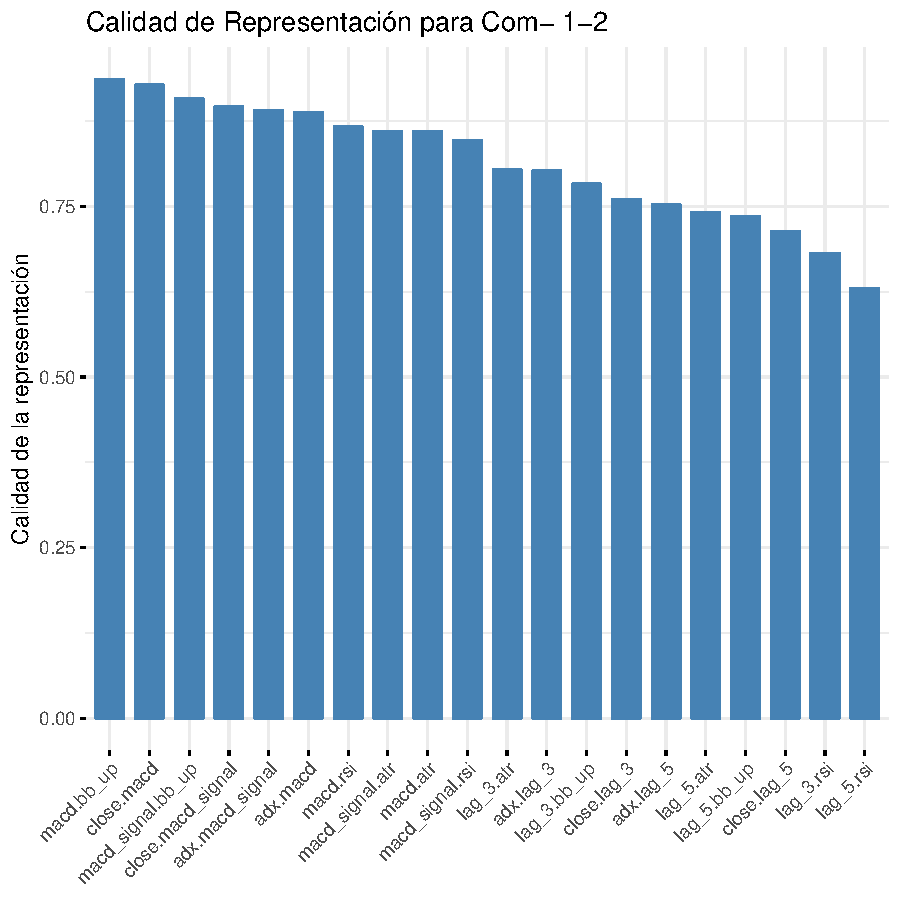
\includegraphics{main-015}
\caption{Calidad de representación medida por $Cos^2$ de cada variable en PC1 y PC2}
\captionof*{table}{Fuente: Cálculos propios}
\end{figure}

El gráfico de correlación ó Factor map muestra la relación entre las variables. Las claves para su interpretación son:

\begin{itemize}
\item Las variables positivamente correlacionadas se encuentran agrupadas entre sí
\item Las variables negativamente correlacionadas se posicionan en cuadrantes opuestos.
\item La distancia entre las variables y el origen mide la calidad de representación de las variables en el gráfico. Mientras más alejado del origen, mejor representadas 
\end{itemize}

\begin{figure}[H]
\setkeys{Gin}{width = 0.8\textwidth}
\centering
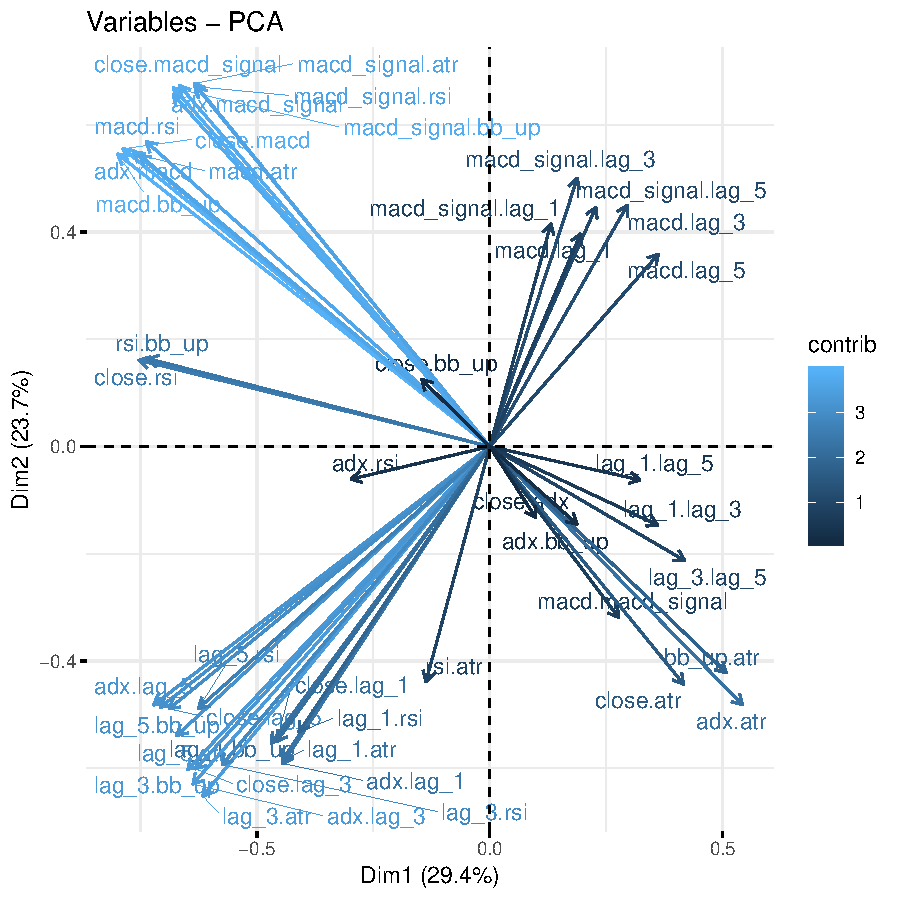
\includegraphics{main-016}
\caption{Gráfico de Correlación entre PC1 y PC2}
\captionof*{table}{Fuente: Cálculos propios}
\end{figure}

En la figura 4.10 se observa el gráfico de correlación para PC1 y PC2, el color de cada variable viene dado por su contribución, mientras más oscuro menor es su contribución a los componentes. Se puede apreciar que las variables con mayor contribución están agrupadas por dos tipos de indicadores predominantes, en el cuadrante superior izquierdo aparecen variables constituidas por interacciones con los indicadores del MACD, mientras que en el cuadrante inferior izquierdo los indicadores predominantes son los rezagos. Se podría resumir que un cuadrante representa la información actual del activo mientras que el otro, la relación entre el precio actual y el precio en períodos anteriores. Por otro lado los grupos forman un ángulo de 90° por lo que no están correlacionados.

En los cuadrantes positivos con respecto al eje x predominan variables con una menor contribución a los componentes. En el cuadrante superior derecho se reflejan las interacciones entre los rezagos y los indicadores del MACD mientras que en el inferior, las interacciones entre los mismos rezagos y otras interacciones con el ATR. Igualmente se observa que las interacciones entre las variables que tienen correlación tienen una menor contribución a los componentes como es el caso de close.bb\_up, adx.rsi, close.adx, entre otros.

Se podría resumir que el cuadrante superior izquierdo esta representado por interacciones del MACD con el precio y con otros indicadores de tendencia y momentum como RSI y ADX. El cuadrante inferior izquierdo las interacciones de los indicadores de tendencia y momentum con los rezagos. El cuadrante superior derecho las interacciones entre el MACD con los rezagos y el cuadrante inferior derecho las interacciones entre indicadores correlacionados.


\begin{figure}[H]
\setkeys{Gin}{width = 0.8\textwidth}
\centering
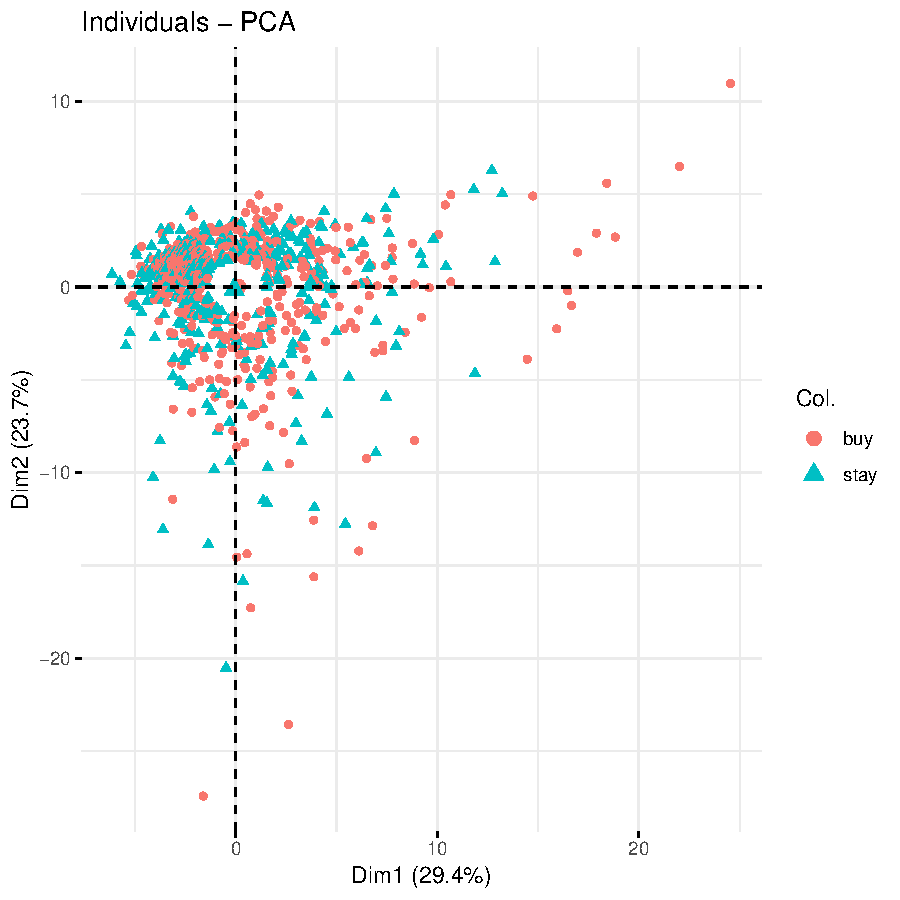
\includegraphics{main-018}
\caption{Gráfico Dispersión entre los componentes. Los puntos rojos representan las observaciones marcadas como 'buys', los triángulos azules los 'stays'}
\captionof*{table}{Fuente: Cálculos propios}
\end{figure}

En la figura 4.11 se muestra el gráfico de dispersión por clases. Se observa que no hay una región que agrupe una sola clase sino que las observaciones están dispersas en todos los cuadrantes, por lo que no es posible hacer un agrupamiento eficientemente.

%%%%%%%%%%%%%%%%%%%%%%%%%%%%%%%%%%%%%%%%%%%%%%%%%%%%%%%%%%%
%%%%%%%%%%%%%%%%%%%%%%%%%%%%%%%%%%%%%%%%%%%%%%%%%%%%%%%%%%%
%%%%%%%%%%%%%%%%%%%%%%%%%%%%%%%%%%%%%%%%%%%%%%%%%%%%%%%%%%%
%%%%%%%%%%%%%%%%%%%%%%%%%%%%%%%%%%%%%%%%%%%%%%%%%%%%%%%%%%%
%%%%%%%%%%%%%%%%%%%%%%%%%%%%%%%%%%%%%%%%%%%%%%%%%%%%%%%%%%%
%%%%%%%%%%%%%%%%%%%%%%%%%%%%%%%%%%%%%%%%%%%%%%%%%%%%%%%%%%%
%%%%%%%%%%%%%%%%%%%%%%%%%%%%%%%%%%%%%%%%%%%%%%%%%%%%%%%%%%%
%%%%%%%%%%%%%%%%%%%%%%%%%%%%%%%%%%%%%%%%%%%%%%%%%%%%%%%%%%%
%%%%%%%%%%%%%%%%%%%%%%%%%%%%%%%%%%%%%%%%%%%%%%%%%%%%%%%%%%%
%%%%%%%%%%%%%%%%%%%%%%%%%%%%%%%%%%%%%%%%%%%%%%%%%%%%%%%%%%%


\newpage

\section{Coeficientes del modelo}

En el presente capítulo se realiza la descripción de los resultados obtenidos después de la aplicación del método propuesto para la estrategia. De igual modo, se presentan los resultados arrojados por las pruebas de Backtesting simulando las entradas y salidas. Los nombres de los componentes fueron sustituidos por etiquetas que intentan explicar la representación del componente en el modelo con ayuda de las gráficas mostradas en la sección 4.1.3.


% pca$x[,1:2] %>% cor()


% list_model[[1]][[1]]$finalModel %>% car::durbinWatsonTest()
% list_model[[1]][[6]]$finalModel %>% car::durbinWatsonTest()
% 
% list_model[[1]][[1]]$finalModel %>% lmtest::dwtest()
% list_model[[1]][[6]]$finalModel %>% lmtest::dwtest()

En la tabla 4.1 se describen los resultados de los coeficientes arrojados por la regresión logística en los 6 períodos de entrenamiento para la serie del S\&P500; en los anexos se muestran el resto de los resultados para los demás índices. Se muestra para cada variable su respectivo coeficiente, así como su error estándar. Se realiza también el contraste Wald - Chi-Cuadrado para verificar la significancia de cada variable en el modelo. Por lo que para cada variable se expone el estadístico z que viene dado por $\beta_{i}/SE(\beta_{i})$ y su respectivo p-valor.

El test Wald - Chi-Cuadrado se puede definir de la siguiente manera:

\begin{itemize}
\item \textbf{$H_{0}$}: $\beta_{i} = 0$
\item \textbf{$H_{i}$}: $\beta_{i} \neq 0$
\item Estadístico de contraste: 

$$Z = \frac{\beta_{i}}{SE(\beta_{i})}$$

\item Nivel de Significación: $\alpha = 5\%$
\item Región Crítica: $p \leq \alpha$
\end{itemize}

\begin{center}
\captionof{table}{Resumen del modelo para cada período de entrenamiento utilizando S\&P500}
\captionof*{table}{Período de entrenamiento 2009 - 2012}
% latex table generated in R 3.6.0 by xtable 1.8-3 package
% Wed May 15 19:22:54 2019
\begin{table}[ht]
\centering
\begin{tabular}{rrrrr}
  \hline
 & Estimate & Std. Error & z value & Pr($>$$|$z$|$) \\ 
  \hline
(Intercept) & -0.36 & 0.06 & -5.56 & 0.00 \\ 
  ATR.Pos-Macd.Neg & -0.01 & 0.02 & -0.81 & 0.42 \\ 
  Macd.Pos-Rezago.Neg & -0.01 & 0.02 & -0.71 & 0.48 \\ 
   \hline
\end{tabular}
\end{table}\end{center}

\begin{center}
\captionof*{table}{Período de entrenamiento 2009 - 2013}
% latex table generated in R 3.6.0 by xtable 1.8-3 package
% Wed May 15 19:22:54 2019
\begin{table}[ht]
\centering
\begin{tabular}{rrrrr}
  \hline
 & Estimate & Std. Error & z value & Pr($>$$|$z$|$) \\ 
  \hline
(Intercept) & -0.41 & 0.06 & -7.04 & 0.00 \\ 
  ATR.Pos-Macd.Neg & 0.02 & 0.02 & 1.33 & 0.18 \\ 
  Macd.Pos-Rezago.Neg & -0.01 & 0.02 & -0.46 & 0.65 \\ 
   \hline
\end{tabular}
\end{table}\end{center}

\newpage
\begin{center}
\captionof*{table}{Período de entrenamiento 2009 - 2014}
% latex table generated in R 3.6.0 by xtable 1.8-3 package
% Wed May 15 19:22:54 2019
\begin{table}[ht]
\centering
\begin{tabular}{rrrrr}
  \hline
 & Estimate & Std. Error & z value & Pr($>$$|$z$|$) \\ 
  \hline
(Intercept) & -0.28 & 0.05 & -5.29 & 0.00 \\ 
  ATR.Pos-Macd.Neg & 0.05 & 0.02 & 2.93 & 0.00 \\ 
  Macd.Pos-Rezago.Neg & 0.02 & 0.02 & 1.39 & 0.16 \\ 
   \hline
\end{tabular}
\end{table}\end{center}

\begin{center}
\captionof*{table}{Período de entrenamiento 2009 - 2015}
% latex table generated in R 3.6.0 by xtable 1.8-3 package
% Wed May 15 19:22:54 2019
\begin{table}[ht]
\centering
\begin{tabular}{rrrrr}
  \hline
 & Estimate & Std. Error & z value & Pr($>$$|$z$|$) \\ 
  \hline
(Intercept) & -0.17 & 0.05 & -3.51 & 0.00 \\ 
  ATR.Pos-Macd.Neg & -0.06 & 0.02 & -4.31 & 0.00 \\ 
  Macd.Pos-Rezago.Neg & 0.02 & 0.02 & 1.21 & 0.23 \\ 
   \hline
\end{tabular}
\end{table}\end{center}

\begin{center}
\captionof*{table}{Período de entrenamiento 2009 - 2016}
% latex table generated in R 3.6.0 by xtable 1.8-3 package
% Wed May 15 19:22:54 2019
\begin{table}[ht]
\centering
\begin{tabular}{rrrrr}
  \hline
 & Estimate & Std. Error & z value & Pr($>$$|$z$|$) \\ 
  \hline
(Intercept) & -0.13 & 0.04 & -2.80 & 0.01 \\ 
  ATR.Pos-Macd.Neg & -0.06 & 0.01 & -4.53 & 0.00 \\ 
  Macd.Pos-Rezago.Neg & 0.03 & 0.01 & 1.76 & 0.08 \\ 
   \hline
\end{tabular}
\end{table}\end{center}

\newpage
\begin{center}
\captionof*{table}{Período de entrenamiento 2009 - 2017}
% latex table generated in R 3.6.0 by xtable 1.8-3 package
% Wed May 15 19:22:54 2019
\begin{table}[ht]
\centering
\begin{tabular}{rrrrr}
  \hline
 & Estimate & Std. Error & z value & Pr($>$$|$z$|$) \\ 
  \hline
(Intercept) & -0.11 & 0.04 & -2.67 & 0.01 \\ 
  ATR.Pos-Macd.Neg & 0.06 & 0.01 & 4.80 & 0.00 \\ 
  Precio.Pos-Rezago.Neg & 0.03 & 0.01 & 2.18 & 0.03 \\ 
   \hline
\end{tabular}
\end{table}\end{center}

Se observa que recién para el tercer período de entrenamiento se obtiene un p-valor menor a 0.05 lo cual indica que el coeficiente es significativo. A medida que la data de entrenamiento es más grande, los coeficientes son más significativos. Se infiere entonces que mientras más observaciones para entrenar el modelo, mayor será la asociación entre los componentes y la capacidad de predecir el retorno objetivo.

También se observa que el signo de los coeficientes varía en las distintas datas de entrenamiento, por ejemplo para el período 2009-2014 ambas variables influyen positivamente en la correcta predicción del retorno objetivo. En los períodos 2009-2015 y 2009-2016 la variable ATR.Pos-Macd.Neg influye negativamente en la variable dependiente caso contrario para la variable Macd.Pos-Rezago.Neg, que influye positivamente.


\begin{figure}[H]
\setkeys{Gin}{height = .5\linewidth, width = .5\linewidth}
\centering
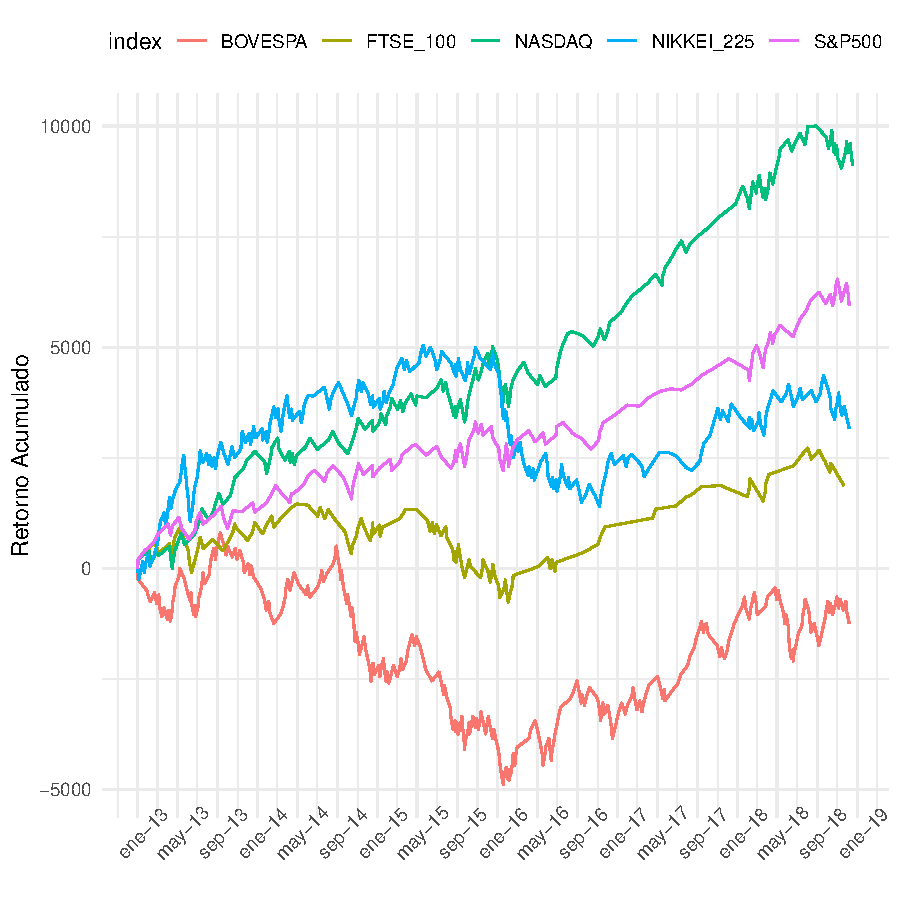
\includegraphics{main-027}
\caption{Gráfico de Dispersión de los p-valores en cada período de entrenamiento}
\captionof*{table}{Fuente: Cálculos propios}
\end{figure}

En los primeros períodos de entrenamiento los coeficientes no son significativos según el test Wald-Chi-Cuadrado. Sin embargo al aumentar el tamaño de los datos de entrenamiento la significancia aumenta en la mayoría de los índices, esto se puede ver reflejado en la figura 4.12. Se observa que los p-valores de los coeficientes de los índices FTSE, NASDAQ y S\&P disminuyen al utilizar mayor data de entrenamiento, caso contrario a los coeficientes de los índices NIKKEI y BOVESPA que pareciera aumentar.

\section{Resultados de la simulación}


\begin{center}
\captionof{table}{Resumen de resultados de aplicar el modelo en la data de prueba para los 5 índices}
% latex table generated in R 3.6.0 by xtable 1.8-3 package
% Wed May 15 19:22:55 2019
\begin{table}[ht]
\centering
\begin{tabular}{cccccc}
  \hline
 & S\&P\_500 & NASDAQ & NIKKEI\_225 & FTSE\_100 & BOVESPA \\ 
  \hline
Compras en Falso & 62 & 72 & 116 & 58 & 141 \\ 
  Compras Verdaderas & 80 & 122 & 153 & 72 & 170 \\ 
  N° transacciones & 142 & 194 & 269 & 130 & 311 \\ 
  Precisión & 56.34\% & 62.89\% & 56.88\% & 55.38\% & 54.66\% \\ 
  Beneficio & 5939.81 & 9101.82 & 3162.62 & 1869.01 & -1250.00 \\ 
   \hline
\end{tabular}
\end{table}\end{center}

En la tabla 4.2 se muestran los resultados de la simulación para cada uno de los índices. Las compras verdaderas son aquellas en las que el modelo predijo una compra y el resultado del trade en la simulación es positivo, en cambio las compras en falso son aquellas en las que el modelo predijo una compra y la transacción resulto en perdida en la simulación. La precisión se mide como el número compras verdaderas divididos por el número de transacciones total. El beneficio se calcula como el monto de ganancia o pérdida arrojada por la simulación

El número de trades cerrados es mayor en los índices BOVESPA y NIKKEI, lo que puede deberse a que estos mercados tuvieron una mayor volatilidad en el período de estudio. Por otra parte la predicción ronda entre 54\% al 62\%, la relación pérdida/ganancia de los parámetros utilizados es $2.5/2 = 1.25$, es decir que por cada trade negativo se necesita 1.25 trades positivos para mitigar la pérdida. En este sentido, una precisión del 60\% asegura un margen de ganancia, sin embargo, el retorno acumulado obtenido es pobre comparado con inversiones pasivas del mismo índice. Además es bastante cercano al 50\% lo que supondría un comportamiento aleatorio del modelo.
 

En la figura 4.12 se observa los trades realizados por la simulación según el resultado de la operación, los trades verdes son aquellos clasificados como 'True buys' y resultaron en ganancia, los rojos, son clasificados como 'False buys' y resultaron en pérdidas y los azules son clasificados como 'False buys' pero cerraron el trade por límite de tiempo.

\begin{figure}[H]
\setkeys{Gin}{height = .7\linewidth, width = .8\textwidth}
\centering
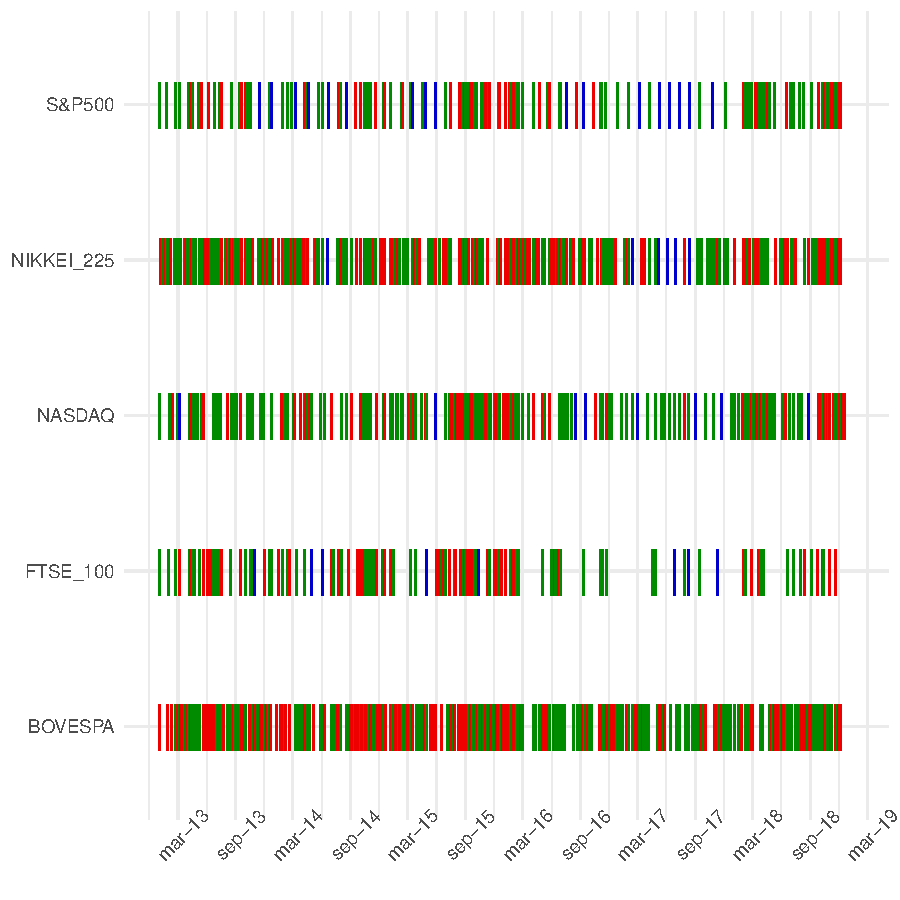
\includegraphics{main-031}
\caption{Clasificación de los trades}
\captionof*{table}{Fuente: Cálculos propios}
\end{figure}

Se observa como en la simulación utilizando el índice BOVESPA, los trades positivos aumentan su frecuencia a partir del segundo semestre del 2016, esto puede deberse al hecho de tener mayor número de observaciones para entrenar el modelo. Igualmente se aprecia como para el S\&P500 las operaciones se concentran en los primeros años de prueba, cerrando los demás años prácticamente sin operaciones.


\begin{figure}[H]
\setkeys{Gin}{width = 1\textwidth}
\centering
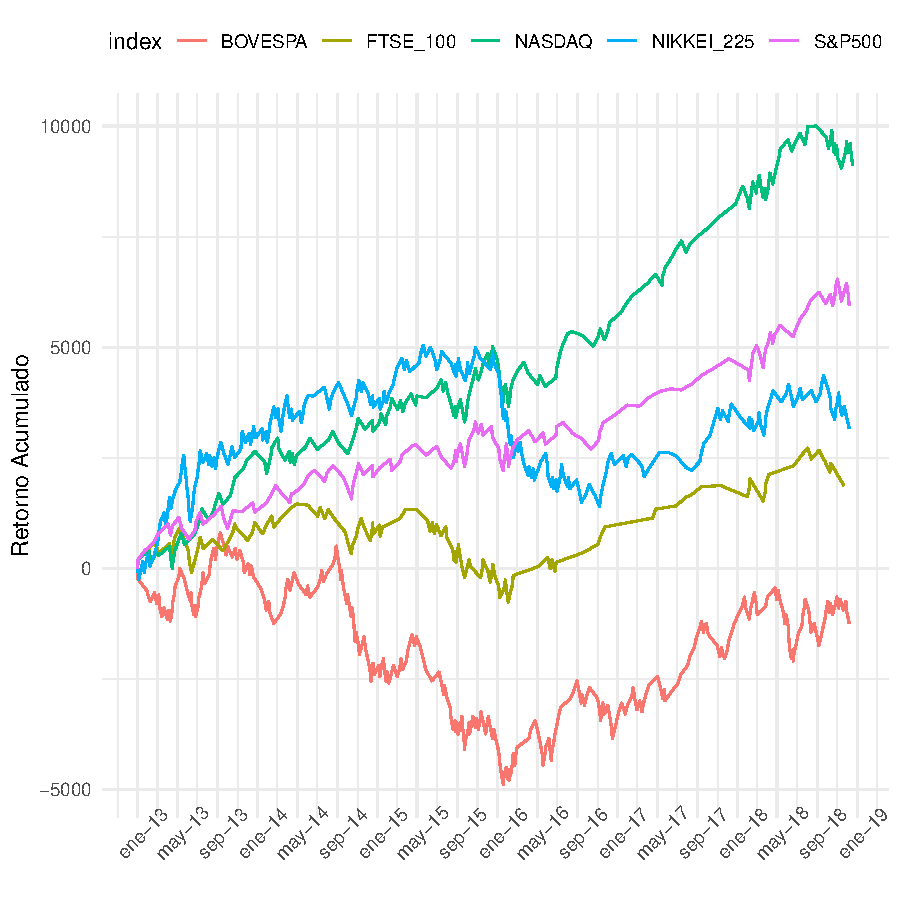
\includegraphics{main-033}
\caption{Retorno acumulado para cada índice}
\captionof*{table}{Fuente: Cálculos propios}
\end{figure}

En la figura 4.13 se observa la curva de capital de las operaciones realizadas con cada uno de los índices. EL NASDAQ y S\&P500 son los de mejor desempeño, mostrando ganancias consistentemente durante todo el período de entrenamiento. Por su lado el NIKKEI y FTSE tienen momentos tanto de ganancia como de pérdida, pero manteniendo un rendimiento positivo. Mientras que el BOVESPA pierde consistentemente durante la primera mitad del período y gana en la segunda mitad, pero terminando con un rendimiento positivo.

\subsection{Backtesting}




\begin{center}
\captionof{table}{Resultados de aplicar el modelo con la metodología backtesting en la data de validación (2016-2018)}
% latex table generated in R 3.6.0 by xtable 1.8-3 package
% Wed May 15 19:23:03 2019
\begin{table}[ht]
\centering
\begin{tabular}{cccccc}
  \hline
 & S\&P\_500 & NASDAQ & NIKKEI\_225 & FTSE\_100 & BOVESPA \\ 
  \hline
Compras en Falso & 31 & 39 & 60 & 16 & 48 \\ 
  Compras Verdaderas & 38 & 55 & 61 & 28 & 74 \\ 
  N° transacciones & 69 & 94 & 121 & 44 & 122 \\ 
  Precisión & 55.07\% & 58.51\% & 50.41\% & 63.64\% & 60.66\% \\ 
  Beneficio & 3081.39 & 3156.77 & -1483.38 & 2234.42 & 2800.00 \\ 
   \hline
\end{tabular}
\end{table}\end{center}

En la tabla 4.13 se exponen a manera de comparación los resultados de la simulación utilizando la metodología convencional de backtesting. Se puede observar que la precisión del modelo es muy parecida a los resultados del walkforward, llegando, incluso a ser mayor para los índices BOVESPA y FTSE. Esto también ocurre debido a que la cantidad de trades es menor en la metodología backtesting ya que se utiliza menor data de validación (2016-2018) en comparación a la metodología walkforward (2013-2018). Sin embargo es un buen indicativo de la pobre efectividad del modelo utilizando esta metodología.

\subsection{Medidas de Riesgo}

Al asumir que siempre se abre la posición con la misma cantidad de dinero, en este caso 10.000 USD, se sabe que los trades sólo pueden arrojar dos resultados 2\% de ganancia en caso que sea positivo ó 2.5\% de pérdida en caso contrario, descartando las liquidaciones por límite de tiempo- En este sentido se aplica el contraste Wald–Wolfowitz comúnmente llamado test de racha, para verificar la aleatoriedad de los resultados de los trades.

La prueba de Wald–Wolfowitz se puede definir de la siguiente manera:

\begin{itemize}
\item \textbf{H0}: La secuencia es producida de manera aleatoria.
\item \textbf{Hi}: La secuencia no es producida de manera aleatoria.
\item Estadístico de contraste: 

$$Z = \frac{R - \mu_{R}}{\sqrt{Var(R)}}$$

donde,

$$\mu_{R} = \frac{2_{n_{1}n_{2}}}{n_{1}+n_{2}}+1  \qquad  Var(R) = \frac{2_{n_{1}n_{2}}(2_{n_{1}n_{2}}-n_{1}-n_{2})}{(n_{1}+n_{2})^{2}(n_{1}+n_{2}-1)}$$

\item Nivel de Significación: $\alpha = 5\%$
\item Región Crítica: $p \leq \alpha$
\end{itemize}

 
\begin{center}
\captionof{table}{Resultados del test de Wald–Wolfowitz (Test de Racha)}
% latex table generated in R 3.6.0 by xtable 1.8-3 package
% Wed May 15 19:23:03 2019
\begin{table}[ht]
\centering
\begin{tabular}{rrr}
  \hline
 & statistic & p.value \\ 
  \hline
S\&P\_500 & -0.28 & 0.78 \\ 
  NASDAQ & 0.60 & 0.55 \\ 
  NIKKEI\_225 & 1.27 & 0.20 \\ 
  FTSE\_100 & 0.37 & 0.71 \\ 
  BOVESPA & -0.25 & 0.81 \\ 
   \hline
\end{tabular}
\end{table}\end{center}

Frente a p-valores mayores a 0.05, y con un nivel de significación del 5\% no existen elementos suficientes para rechazar la hipótesis nula de aleatoriedad en la secuencia de los resultados de los trades, por lo que se puede concluir que los trades son independientes. Esta independencia permite asumir que la suma de las variables al tener una muestra suficientemente grande, se distribuye N(0, 1). Se calcula entonces el VaR y ES para cada una de las estrategias.


\newpage
\begin{center}
\captionof{table}{VaR y ES para retornos de cada índice}
% latex table generated in R 3.6.0 by xtable 1.8-3 package
% Wed May 15 19:23:03 2019
\begin{table}[ht]
\centering
\begin{tabular}{rlllll}
  \hline
 & S\&P\_500 & NASDAQ & NIKKEI\_225 & FTSE\_100 & BOVESPA \\ 
  \hline
VaR & 6,297.49 & 5,622.23 & 6,246.23 & 6,386.23 & 6,451.87 \\ 
  ES & 7,912.80 & 7,195.66 & 7,859.20 & 8,005.20 & 8,073.22 \\ 
   \hline
\end{tabular}
\end{table}\end{center}
  
Se puede observar en la tabla 4.4 como el VaR para cada estrategia varía en función de la precisión del modelo, como es de esperar. Para los índices con mayor precisión el VaR es menor y por lo tanto también lo es el ES. En este sentido se puede interpretar el VaR y ES del S\&P500 como: 'Cuando la estrategia toma como activo el índice S\&P500, existe una probabilidad del 5\% de que genere una pérdida igual ó mayor a 6,297.49 USD luego de 300 trades realizados. En caso de que ocurra una pérdida mayor, se espera que el déficit total sea de 7,912.80 USD'
% !TeX root = ./main.Rnw
%\SweaveUTF8

\chapter*{Conclusiones y Recomendaciones}
\addcontentsline{toc}{chapter}{Conclusiones y Recomendaciones}

En esta investigación se ha planteado un marco de trabajo que permite el desarrollo y prueba para una estrategia de trading automatizado. Se busca demostrar que es posible obtener rendimientos positivos con una estrategia basada en indicadores técnicos, utilizados como variables predictoras en un modelo de aprendizaje automático. El modelo arrojo una precisión para todos los índices de entre el 54\% y 63\%, estos valores concuerdan con los resultados de otras investigaciones que utilizan modelos lineales en los mismos activos. 

Ahora bien, los resultados arrojados no generan suficiente confianza como para concluir que es posible pronosticar movimientos del mercado con este tipo de modelo. Particularmente, el enfoque de buscar incrementos porcentuales es sensible a los parámetros de Take Profit y Stop Loss, por lo que, su estandarización a 2\% y 2.5\% respectivamente puede ser una gran limitante del modelo. Si bien se intentó optimizar estos valores, los resultados en los datos de prueba no fueron concluyentes.

Por otro lado, al observar los gráficos de correlación entre los componentes del ACP, en la mayoría de los casos se observan dos grupos que aportan la mayor cantidad de información; uno de los grupos está dominado por las interacciones del MACD, y el segundo por las interacciones de los rezagos. Normalmente estos grupos forman un ángulo de 90° pero poseen el mismo signo en cuanto al eje x -componente con mayor información-. Esto deja ver que aún utilizando un número considerable de indicadores, la información que proporcionan al modelo no es suficiente para obtener una precisión aceptable. 

Otras de las limitantes fue la cantidad de observaciones a utilizar, se observó que en tres de los cinco índices el p-valor del test Wald - Chi-Cuadrado disminuye mientras más años de entrenamiento se utiliza, concluyendo, que con mayor cantidad de datos las variables son más significativas para el modelo.

En los resultados no se contemplan las comisiones acarreadas por la operación. Se asume también, que siempre se logra comprar la cantidad establecida en el precio de cierre de la vela, hecho que no siempre ocurre sobre todo en mercados de alta volatilidad y poca liquidez. Si bien el retorno acumulado durante 6 años de prueba es poco atractivo, se sabe que en la práctica los fondos utilizan los futuros como activos de inversión, estos permiten un apalancamiento en el riesgo, lo cual se traduce en mover altos volúmenes de dinero con una posición menor que la que se necesitaría en el mercado de acciones. De cualquier manera los resultados de la precisión dejan ver la posibilidad de un amplio rango de mejora en el performance de la estrategia. 

Este modelo puede ser mejorado de muchas maneras, incluyendo, por ejemplo la optimización de los parámetros Take Profit, Stop Loss para el activo a operar, así como la elección del tamaño de los períodos de entrenamiento ó el número de componentes a utilizar como variables predictoras. Otras de las limitaciones presente es el de utilizar un modelo lineal, si bien se decide utilizar MLG como punto de partida es muy probable que algún modelo que no asuma linealidad como Bosques Aleatorios, SVM ó Redes Neuronales mejoren la predicción. 

El modelo solo considera la prediccion del incremento del precio. Se utiliza la figura del stop loss como reduccion del riesgo. Un alternativa para obtener protección podría ser invertir el modelo, es decir predecir una disminución del precio, de esta manera se podría dejar de lado el stop loss y liquidar la posición cuando el modelo prediga una disminución en los precios.

Otra posible fuente de optimización podría ser la elección de los indicadores técnicos. Se podría profundizar en el aspecto técnico para su elección y el de las configuraciones de los mismos buscando mejorar la predicción del modelo. De cualquier manera este proyecto busca ser un punto de partida para futuras investigaciones.


% !TeX root = ./main.Rnw
%\SweaveUTF8

\chapter{Anexos}

\section{Coeficientes de los modelos}

\begin{center}
\captionof{table}{Resumen del modelo para cada período de entrenamiento utilizando NASDAQ}
\captionof*{table}{Período de entrenamiento 2009 - 2012}
% latex table generated in R 3.6.0 by xtable 1.8-3 package
% Wed May 15 19:23:03 2019
\begin{table}[ht]
\centering
\begin{tabular}{rrrrr}
  \hline
 & Estimate & Std. Error & z value & Pr($>$$|$z$|$) \\ 
  \hline
(Intercept) & -0.3127 & 0.0638 & -4.90 & 0.0000 \\ 
  PC1 & -0.0021 & 0.0179 & -0.12 & 0.9068 \\ 
  PC2 & 0.0058 & 0.0201 & 0.29 & 0.7718 \\ 
   \hline
\end{tabular}
\end{table}\end{center}

\begin{center}
\captionof*{table}{Período de entrenamiento 2009 - 2013}
% latex table generated in R 3.6.0 by xtable 1.8-3 package
% Wed May 15 19:23:03 2019
\begin{table}[ht]
\centering
\begin{tabular}{rrrrr}
  \hline
 & Estimate & Std. Error & z value & Pr($>$$|$z$|$) \\ 
  \hline
(Intercept) & -0.3667 & 0.0574 & -6.39 & 0.0000 \\ 
  PC1 & 0.0124 & 0.0164 & 0.75 & 0.4524 \\ 
  PC2 & 0.0001 & 0.0184 & 0.00 & 0.9978 \\ 
   \hline
\end{tabular}
\end{table}\end{center}
\begin{center}
\captionof*{table}{Período de entrenamiento 2009 - 2014}
% latex table generated in R 3.6.0 by xtable 1.8-3 package
% Wed May 15 19:23:03 2019
\begin{table}[ht]
\centering
\begin{tabular}{rrrrr}
  \hline
 & Estimate & Std. Error & z value & Pr($>$$|$z$|$) \\ 
  \hline
(Intercept) & -0.3027 & 0.0522 & -5.80 & 0.0000 \\ 
  PC1 & 0.0291 & 0.0153 & 1.91 & 0.0565 \\ 
  PC2 & -0.0203 & 0.0170 & -1.20 & 0.2318 \\ 
   \hline
\end{tabular}
\end{table}\end{center}

\newpage

\begin{center}
\captionof*{table}{Período de entrenamiento 2009 - 2015}
% latex table generated in R 3.6.0 by xtable 1.8-3 package
% Wed May 15 19:23:03 2019
\begin{table}[ht]
\centering
\begin{tabular}{rrrrr}
  \hline
 & Estimate & Std. Error & z value & Pr($>$$|$z$|$) \\ 
  \hline
(Intercept) & -0.2748 & 0.0483 & -5.69 & 0.0000 \\ 
  PC1 & 0.0524 & 0.0148 & 3.55 & 0.0004 \\ 
  PC2 & -0.0238 & 0.0158 & -1.51 & 0.1303 \\ 
   \hline
\end{tabular}
\end{table}\end{center}

\begin{center}
\captionof*{table}{Período de entrenamiento 2009 - 2016}
% latex table generated in R 3.6.0 by xtable 1.8-3 package
% Wed May 15 19:23:03 2019
\begin{table}[ht]
\centering
\begin{tabular}{rrrrr}
  \hline
 & Estimate & Std. Error & z value & Pr($>$$|$z$|$) \\ 
  \hline
(Intercept) & -0.2641 & 0.0451 & -5.85 & 0.0000 \\ 
  PC1 & -0.0426 & 0.0136 & -3.13 & 0.0018 \\ 
  PC2 & 0.0291 & 0.0148 & 1.97 & 0.0484 \\ 
   \hline
\end{tabular}
\end{table}\end{center}
\begin{center}
\captionof*{table}{Período de entrenamiento 2009 - 2017}
% latex table generated in R 3.6.0 by xtable 1.8-3 package
% Wed May 15 19:23:03 2019
\begin{table}[ht]
\centering
\begin{tabular}{rrrrr}
  \hline
 & Estimate & Std. Error & z value & Pr($>$$|$z$|$) \\ 
  \hline
(Intercept) & -0.3420 & 0.0428 & -8.00 & 0.0000 \\ 
  PC1 & 0.0358 & 0.0129 & 2.78 & 0.0055 \\ 
  PC2 & -0.0323 & 0.0143 & -2.26 & 0.0240 \\ 
   \hline
\end{tabular}
\end{table}\end{center}

\newpage

\begin{center}
\captionof{table}{Resumen del modelo para cada período de entrenamiento utilizando NIKKEI 225}
\captionof*{table}{Período de entrenamiento 2009 - 2012}
% latex table generated in R 3.6.0 by xtable 1.8-3 package
% Wed May 15 19:23:03 2019
\begin{table}[ht]
\centering
\begin{tabular}{rrrrr}
  \hline
 & Estimate & Std. Error & z value & Pr($>$$|$z$|$) \\ 
  \hline
(Intercept) & -0.2532 & 0.0645 & -3.92 & 0.0001 \\ 
  PC1 & -0.0169 & 0.0173 & -0.97 & 0.3297 \\ 
  PC2 & -0.0255 & 0.0217 & -1.18 & 0.2393 \\ 
   \hline
\end{tabular}
\end{table}\end{center}

\begin{center}
\captionof*{table}{Período de entrenamiento 2009 - 2013}
% latex table generated in R 3.6.0 by xtable 1.8-3 package
% Wed May 15 19:23:03 2019
\begin{table}[ht]
\centering
\begin{tabular}{rrrrr}
  \hline
 & Estimate & Std. Error & z value & Pr($>$$|$z$|$) \\ 
  \hline
(Intercept) & -0.3273 & 0.0580 & -5.64 & 0.0000 \\ 
  PC1 & -0.0260 & 0.0154 & -1.69 & 0.0908 \\ 
  PC2 & -0.0118 & 0.0195 & -0.61 & 0.5438 \\ 
   \hline
\end{tabular}
\end{table}\end{center}

\begin{center}
\captionof*{table}{Período de entrenamiento 2009 - 2014}
% latex table generated in R 3.6.0 by xtable 1.8-3 package
% Wed May 15 19:23:03 2019
\begin{table}[ht]
\centering
\begin{tabular}{rrrrr}
  \hline
 & Estimate & Std. Error & z value & Pr($>$$|$z$|$) \\ 
  \hline
(Intercept) & -0.3303 & 0.0529 & -6.24 & 0.0000 \\ 
  PC1 & -0.0154 & 0.0142 & -1.08 & 0.2784 \\ 
  PC2 & -0.0130 & 0.0177 & -0.74 & 0.4609 \\ 
   \hline
\end{tabular}
\end{table}\end{center}

\newpage

\begin{center}
\captionof*{table}{Período de entrenamiento 2009 - 2015}
% latex table generated in R 3.6.0 by xtable 1.8-3 package
% Wed May 15 19:23:03 2019
\begin{table}[ht]
\centering
\begin{tabular}{rrrrr}
  \hline
 & Estimate & Std. Error & z value & Pr($>$$|$z$|$) \\ 
  \hline
(Intercept) & -0.3038 & 0.0489 & -6.21 & 0.0000 \\ 
  PC1 & -0.0008 & 0.0135 & -0.06 & 0.9529 \\ 
  PC2 & -0.0087 & 0.0166 & -0.52 & 0.6022 \\ 
   \hline
\end{tabular}
\end{table}\end{center}

\begin{center}
\captionof*{table}{Período de entrenamiento 2009 - 2016}
% latex table generated in R 3.6.0 by xtable 1.8-3 package
% Wed May 15 19:23:03 2019
\begin{table}[ht]
\centering
\begin{tabular}{rrrrr}
  \hline
 & Estimate & Std. Error & z value & Pr($>$$|$z$|$) \\ 
  \hline
(Intercept) & -0.2830 & 0.0457 & -6.20 & 0.0000 \\ 
  PC1 & 0.0091 & 0.0129 & 0.70 & 0.4823 \\ 
  PC2 & -0.0075 & 0.0154 & -0.48 & 0.6290 \\ 
   \hline
\end{tabular}
\end{table}\end{center}
\begin{center}
\captionof*{table}{Período de entrenamiento 2009 - 2017}
% latex table generated in R 3.6.0 by xtable 1.8-3 package
% Wed May 15 19:23:03 2019
\begin{table}[ht]
\centering
\begin{tabular}{rrrrr}
  \hline
 & Estimate & Std. Error & z value & Pr($>$$|$z$|$) \\ 
  \hline
(Intercept) & -0.2731 & 0.0427 & -6.39 & 0.0000 \\ 
  PC1 & -0.0000 & 0.0120 & -0.00 & 0.9989 \\ 
  PC2 & 0.0016 & 0.0145 & 0.11 & 0.9093 \\ 
   \hline
\end{tabular}
\end{table}\end{center}

\newpage

\begin{center}
\captionof{table}{Resumen del modelo para cada período de entrenamiento utilizando FTSE 100}
\captionof*{table}{Período de entrenamiento 2009 - 2012}
% latex table generated in R 3.6.0 by xtable 1.8-3 package
% Wed May 15 19:23:03 2019
\begin{table}[ht]
\centering
\begin{tabular}{rrrrr}
  \hline
 & Estimate & Std. Error & z value & Pr($>$$|$z$|$) \\ 
  \hline
(Intercept) & -0.1520 & 0.0633 & -2.40 & 0.0164 \\ 
  PC1 & -0.0369 & 0.0178 & -2.08 & 0.0379 \\ 
  PC2 & -0.0072 & 0.0199 & -0.36 & 0.7184 \\ 
   \hline
\end{tabular}
\end{table}\end{center}

\begin{center}
\captionof*{table}{Período de entrenamiento 2009 - 2013}
% latex table generated in R 3.6.0 by xtable 1.8-3 package
% Wed May 15 19:23:03 2019
\begin{table}[ht]
\centering
\begin{tabular}{rrrrr}
  \hline
 & Estimate & Std. Error & z value & Pr($>$$|$z$|$) \\ 
  \hline
(Intercept) & -0.1554 & 0.0567 & -2.74 & 0.0061 \\ 
  PC1 & 0.0390 & 0.0160 & 2.43 & 0.0150 \\ 
  PC2 & 0.0234 & 0.0181 & 1.29 & 0.1956 \\ 
   \hline
\end{tabular}
\end{table}\end{center}
\begin{center}
\captionof*{table}{Período de entrenamiento 2009 - 2014}
% latex table generated in R 3.6.0 by xtable 1.8-3 package
% Wed May 15 19:23:03 2019
\begin{table}[ht]
\centering
\begin{tabular}{rrrrr}
  \hline
 & Estimate & Std. Error & z value & Pr($>$$|$z$|$) \\ 
  \hline
(Intercept) & -0.0390 & 0.0518 & -0.75 & 0.4517 \\ 
  PC1 & -0.0570 & 0.0149 & -3.82 & 0.0001 \\ 
  PC2 & -0.0481 & 0.0167 & -2.88 & 0.0040 \\ 
   \hline
\end{tabular}
\end{table}\end{center}

\newpage

\begin{center}
\captionof*{table}{Período de entrenamiento 2009 - 2015}
% latex table generated in R 3.6.0 by xtable 1.8-3 package
% Wed May 15 19:23:03 2019
\begin{table}[ht]
\centering
\begin{tabular}{rrrrr}
  \hline
 & Estimate & Std. Error & z value & Pr($>$$|$z$|$) \\ 
  \hline
(Intercept) & 0.0475 & 0.0481 & 0.99 & 0.3228 \\ 
  PC1 & -0.0724 & 0.0140 & -5.19 & 0.0000 \\ 
  PC2 & -0.0369 & 0.0151 & -2.44 & 0.0149 \\ 
   \hline
\end{tabular}
\end{table}\end{center}

\begin{center}
\captionof*{table}{Período de entrenamiento 2009 - 2016}
% latex table generated in R 3.6.0 by xtable 1.8-3 package
% Wed May 15 19:23:03 2019
\begin{table}[ht]
\centering
\begin{tabular}{rrrrr}
  \hline
 & Estimate & Std. Error & z value & Pr($>$$|$z$|$) \\ 
  \hline
(Intercept) & -0.0138 & 0.0449 & -0.31 & 0.7592 \\ 
  PC1 & -0.0648 & 0.0130 & -4.98 & 0.0000 \\ 
  PC2 & -0.0444 & 0.0143 & -3.10 & 0.0019 \\ 
   \hline
\end{tabular}
\end{table}\end{center}
\begin{center}
\captionof*{table}{Período de entrenamiento 2009 - 2017}
% latex table generated in R 3.6.0 by xtable 1.8-3 package
% Wed May 15 19:23:03 2019
\begin{table}[ht]
\centering
\begin{tabular}{rrrrr}
  \hline
 & Estimate & Std. Error & z value & Pr($>$$|$z$|$) \\ 
  \hline
(Intercept) & 0.0372 & 0.0424 & 0.88 & 0.3809 \\ 
  PC1 & -0.0730 & 0.0125 & -5.86 & 0.0000 \\ 
  PC2 & -0.0520 & 0.0137 & -3.81 & 0.0001 \\ 
   \hline
\end{tabular}
\end{table}\end{center}

\newpage

\begin{center}
\captionof{table}{Resumen del modelo para cada período de entrenamiento utilizando BOVESPA}
\captionof*{table}{Período de entrenamiento 2009 - 2012}
% latex table generated in R 3.6.0 by xtable 1.8-3 package
% Wed May 15 19:23:03 2019
\begin{table}[ht]
\centering
\begin{tabular}{rrrrr}
  \hline
 & Estimate & Std. Error & z value & Pr($>$$|$z$|$) \\ 
  \hline
(Intercept) & -0.2403 & 0.0641 & -3.75 & 0.0002 \\ 
  PC1 & -0.0190 & 0.0174 & -1.09 & 0.2750 \\ 
  PC2 & -0.0089 & 0.0219 & -0.41 & 0.6849 \\ 
   \hline
\end{tabular}
\end{table}\end{center}


\begin{center}
\captionof*{table}{Período de entrenamiento 2009 - 2013}
% latex table generated in R 3.6.0 by xtable 1.8-3 package
% Wed May 15 19:23:03 2019
\begin{table}[ht]
\centering
\begin{tabular}{rrrrr}
  \hline
 & Estimate & Std. Error & z value & Pr($>$$|$z$|$) \\ 
  \hline
(Intercept) & -0.1491 & 0.0570 & -2.61 & 0.0089 \\ 
  PC1 & -0.0152 & 0.0154 & -0.98 & 0.3262 \\ 
  PC2 & -0.0183 & 0.0196 & -0.93 & 0.3503 \\ 
   \hline
\end{tabular}
\end{table}\end{center}
\begin{center}
\captionof*{table}{Período de entrenamiento 2009 - 2014}
% latex table generated in R 3.6.0 by xtable 1.8-3 package
% Wed May 15 19:23:03 2019
\begin{table}[ht]
\centering
\begin{tabular}{rrrrr}
  \hline
 & Estimate & Std. Error & z value & Pr($>$$|$z$|$) \\ 
  \hline
(Intercept) & -0.1055 & 0.0517 & -2.04 & 0.0414 \\ 
  PC1 & -0.0134 & 0.0141 & -0.95 & 0.3435 \\ 
  PC2 & -0.0186 & 0.0176 & -1.06 & 0.2905 \\ 
   \hline
\end{tabular}
\end{table}\end{center}

\newpage

\begin{center}
\captionof*{table}{Período de entrenamiento 2009 - 2015}
% latex table generated in R 3.6.0 by xtable 1.8-3 package
% Wed May 15 19:23:03 2019
\begin{table}[ht]
\centering
\begin{tabular}{rrrrr}
  \hline
 & Estimate & Std. Error & z value & Pr($>$$|$z$|$) \\ 
  \hline
(Intercept) & -0.0741 & 0.0478 & -1.55 & 0.1209 \\ 
  PC1 & 0.0120 & 0.0130 & 0.92 & 0.3564 \\ 
  PC2 & -0.0103 & 0.0162 & -0.63 & 0.5268 \\ 
   \hline
\end{tabular}
\end{table}\end{center}

\begin{center}
\captionof*{table}{Período de entrenamiento 2009 - 2016}
% latex table generated in R 3.6.0 by xtable 1.8-3 package
% Wed May 15 19:23:03 2019
\begin{table}[ht]
\centering
\begin{tabular}{rrrrr}
  \hline
 & Estimate & Std. Error & z value & Pr($>$$|$z$|$) \\ 
  \hline
(Intercept) & -0.1257 & 0.0447 & -2.81 & 0.0049 \\ 
  PC1 & 0.0096 & 0.0120 & 0.80 & 0.4229 \\ 
  PC2 & -0.0063 & 0.0154 & -0.41 & 0.6798 \\ 
   \hline
\end{tabular}
\end{table}\end{center}
\begin{center}
\captionof*{table}{Período de entrenamiento 2009 - 2017}
% latex table generated in R 3.6.0 by xtable 1.8-3 package
% Wed May 15 19:23:03 2019
\begin{table}[ht]
\centering
\begin{tabular}{rrrrr}
  \hline
 & Estimate & Std. Error & z value & Pr($>$$|$z$|$) \\ 
  \hline
(Intercept) & -0.1851 & 0.0423 & -4.38 & 0.0000 \\ 
  PC1 & 0.0068 & 0.0113 & 0.60 & 0.5489 \\ 
  PC2 & -0.0043 & 0.0145 & -0.30 & 0.7675 \\ 
   \hline
\end{tabular}
\end{table}\end{center}

% !TeX root = ./main.Rnw
%\SweaveUTF8

\chapter*{Referencias}
\addcontentsline{toc}{chapter}{Referencias}

\begin{itemize}

\item Abdi H. \& Williams L. (2010) \textit{Principal Component Analysis}. Estados Unidos: John Wiley \& Sons. Recuperado de: http://www.utdallas.edu/~herve/abdi-awPCA2010.pdf

\item Abhijit, G. (2017). \textit{Machine Learning with R}. Singapur: Springer.

\item Araneda, H (2015). \textit{Diseño e Implementación de un Sistema Automatizado Para Operar en el Mercado de Divisas Usando Reglas de Asociación}. (Tesis de Master). Universidad de Chile, Chile.

\item Bach, W. \& Nielsen, K. (2018). \textit{On Machine Learning Based Cryptocurrency Trading}. (Tesis de Master). Aalborg University, Dinamarca.

\item Balestrini, M. (1997). \textit{Como se Elabora el Proyecto de Investigación}. BL Consultores y Asociados: Venezuela.

\item Comité de Supervisión Bancaria de Basilea. (2016) \textit{Requerimientos mínimos de capital por riesgo de mercado} Recuperado de: https://www.bis.org/bcbs/publ/d352\_es.pdf

\item Danielsson, J. (2011). \textit{Financial Risk Forecasting}. Reino Unido: Wiley.

\item Day, T. \& Wang, P. (2002), \textit{Dividends, Nonsynchronous Prices, and the Returns from Trading the Dow Jones Industrial Average} Journal of Empirical Finance, 9, 431-454.

\item Fernández, C. (2008). \textit{Modelos Ocultos de Markov Aplicados al Reconocimiento de Patrones del Análisis Técnico Búrsatil}. Universidad Nacional de Córdoba, Argentina.

\item Froot, K., Scharfstein, S. \& Stein, J. (1992), \textit{Herd on the Street: Informational Inefficiencies in a Market with Short-Term Speculation}. Journal of Finance, 47, 1461-1484.

\item González, L. (2002). \textit{Análisis Financiero del Portafolio Mercantil de Inversión de MERINVEST. Período 1998-2000}. (Tesis de Postgrado). Universidad Católica Andrés Bello, Venezuela.

\item Hong, H. \& Stein, J. (1999) \textit{A Unified Theory of Underreaction, Momentum Trading, and Overreaction in Asset Markets}. Journal of Finance, 6, 2143-2147.

\item Huertas, L. (2015). \textit{Modelos Predictivos para el mercado FOREX}. (Tesis de Master). Universidad de Murcia, España.

\item Investopedia. (1999-2019). \textit{Diccionario de Términos}. New York, NY. http://www.investopedia.com

\item James, G., Witten D., Hastie, T., \& Tibshirani. R. (2013). \textit{An Introduction to Statistical Learning}. Londres: Springer.

\item Lu, N. (2016). \textit{A machine Learning Approach to Automated Trading}. (Tesis de Postgrado). Boston College Computer Science, Estados Unidos.

\item Mitchell, T. (1997) \textit{Machine Learning}. Estados Unidos: McGraw-Hill

\item Murphy, J. (1999). \textit{Análisis Técnico de los Mercados Financieros}. New York: Gestión 2000.

\item Pfaff, B. (2016). \textit{Financial Risk Modelling and Portfolio Optimization with R}. Reino Unido: Wiley.

\item Rebolledo, V. (2018). \textit{Evaluación de la Efectividad del Método GARCH-EVT-COPULAS para el Cálculo del VaR como Medida de Riesgo en Mercados de Commodities Latinoamericanos}. (Tesis de Pregrado). Universidad Central de Venezuela, Venezuela.

\item Robert, R. (2008) \textit{Wall Street The Markets, Mechanisms and Players}. Estados Unidos: The Economist

\item Seijas, F. (1993). \textit{Investigación por muestreo}. Ediciones Fabreton: Venezuela.

\item Shagilla, K. (2006). \textit{An Analysis of Technical Trading Strategies}. (Tesis de Doctorado). Leeds University Business School, Inglaterra.

\item The Balance. (1999-2019). \textit{Diccionario de Términos}. New York, NY. http://www.thebalance.com

\item Udacity. (Productor). (2018-2019). \textit{Machine Learning for Trading} [WEB]. https://www.udacity.com

\end{itemize}

\end{document}
